%
% Template for Doctoral Theses at Uppsala 
% University. The template is based on    
% the layout and typography used for      
% dissertations in the Acta Universitatis 
% Upsaliensis series                      
% Ver 5.2 - 2012-08-08                  
% Latest version available at:            
%   http://ub.uu.se/thesistemplate            
%                                         
% Support: Wolmar Nyberg Akerstrom        
% Thesis Production           
% Uppsala University Library              
% avhandling@ub.uu.se                          
%                                         
%%%%%%%%%%%%%%%%%%%%%%%%%%%%%%%%%%%%%%%%%%%


\documentclass{UUThesisTemplate}

% Package to determine wether XeTeX is used
\usepackage{ifxetex}
\usepackage{mathtools}
\newcommand\isdef{\stackrel{\mathclap{\tiny\normalfont\mbox{def}}}{=}}
\ifxetex
	% XeTeX specific packages and settings
	% Language, diacritics and hyphenation
	\usepackage[babelshorthands]{polyglossia}
	\setmainlanguage{english}
	\setotherlanguages{swedish}

	% Font settings
	\setmainfont{Times New Roman}
	\setromanfont{Times New Roman}
	\setsansfont{Arial}
	\setmonofont{Courier New}
\else
	% Plain LaTeX specific packages and settings
	% Language, diacritics and hyphenation
    % Use English and Swedish languages. 
	\usepackage[swedish,english]{babel} 

	% Font settings
	\usepackage{type1cm}
	\usepackage[utf8]{inputenc}
	\usepackage[T1]{fontenc}
	\usepackage{mathptmx}
	
	% Enable scaling of images on import
	\usepackage{graphicx}
\fi


% Tables
\usepackage{booktabs}
\usepackage{tabularx}

% Document links and bookmarks
\usepackage{hyperref} 

% Numbering of headings down to the subsection level
\numberingdepth{section}

% Including headings down to the subsection level in contents
\contentsdepth{section}


% Uncomment to use a custom abstract dummy text
%\abstractdummy{
%	\begin{abstract}
%		Please use no more than 300 words and avoid mathematics or complex script.
%	\end{abstract}
%}


\begin{document}
\frontmatter
    % Creates the front matter (title page(s), abstract, list of papers)
    % for either a Comprehensive Summary or a Monograph.
    % Authors of Comprehensive Summaries use this front matter 
    \frontmatterCS 
    % Monograph authors use this front matter 
    %\frontmatterMonograph 
 
   % Optional dedication
   \dedication{Dedicated to new Life: Emmanuel and Mathis}
 
    % Environment used to create a list of papers
    \begin{listofpapers}
    	\item \textbf{van der Schot, G} et al. Imaging single cells in a beam of live cyanobacteria. \textit{Nature Communications} \textbf{6}, 5704 (2015). %\label{ImCell}
        \item \textbf{van der Schot, G} et al. Open dataset of live cyanobacterial cells imaged using an X-ray laser. \textit{Nature Scientific Data} \textbf{3},  160064 (2016)%\label{DataCell}
        %\item \textbf{van der Schot, G} et al. RedFlamingo: Suite for automated classification of diffraction patterns. \textit{in preparation }%\label{RedFlamingo}
        \item Munke, A., \textbf{van der Schot, G} et al. Open dataset of RDV particles. \textit{in preparation} %\label{DataRDV}
        
    \end{listofpapers}
    
    \begin{listofsupportingpapers}
	\item G. van der Schot and A.M.J.J. Bonvin. Performance of the WeNMR CS-Rosetta3 web server in CASD-NMR. Journal of Biomolecular NMR, 62(4),497-502, 2015.	
	\item G. van der Schot \textit{et al.} Improving 3D structure prediction from chemical shift data. Journal of biomolecular NMR, 57(1):27-35,2013.
	\item T.A. Wassenaar \textit{et al.} WeNMR: Structural Biology on the Grid. Journal of Grid Computing, 10(4):747-767, 2012.
	\item A. Rosato    \textit{et al.} Blind testing of routine, fully automated determination of protein structures from NMR data. Structure, 20(2):227-236, 2012.
	\item M. Vendruscolo \textit{et al.} Protein structure
determination using chemical shifts, NMR in Mechanistic Systems Biology, Chapter 10, 107-110, 2009.
 	\item A. Rosato    \textit{et al.} CASD-NMR: critical assessment of automated structure determination by NMR. Nature Methods, 6(9):625-626, 2009.
 	\item T. Gorkhover Femtosecond X-ray Fourier holography imaging of free-flying nanoparticles. Nature Photonics \textit{Accepted}
 	\item R.P. Kurta   \textit{et al.} Correlations in scattered x-ray laser pulses reveal nanoscale structural features of viruses. Phys. Rev. Lett. 119, 158102, 2017.
	\item H.K.N. Reddy \textit{et al.} Coherent soft X$-$ray diffraction imaging of coliphage PR772 at the Linac coherent light source. Scientific Data, 4:170079, 2017.
	\item  B.J. Daurer \textit{et al.} Experimental strategies for imaging bioparticles with femtosecond hard X-ray pulses. IUCrJ, 4(3):252-262, 2017.
	\item M.F. Hantke  \textit{et al.} A data set from flash X-ray imaging of carboxysomes. Scientific data, 3:160061, aug 2016.
	\item A. Munke     \textit{et al.} Coherent diffraction of single Rice Dwarf virus particles using hard X-rays at the Linac Coherent Light Source. Scientific data, 3:160064, 2016.
	\item T. Ekeberg   \textit{et al.} Three-Dimensional Reconstruction of the Giant Mimivirus Particle with an X-Ray Free-Electron Laser. Physical Review Letters, 114(9):098102, 2015.
	\item M.F. Hantke  \textit{et al.} High-throughput imaging of heterogeneous cell organelles with an X-ray laser. Nature Photonics, 8(12):943-949, 2014.
	\item A.V. Martin  \textit{et al.} Noise-robust coherent diffractive imaging with a single diffraction pattern. Optics Express, 20(15):16650, 2012.	
    \end{listofsupportingpapers}
    \begingroup
        % To adjust the indentation in your table of contents, uncomment and enter the widest numbers for each level
        %  E.g.  \settocnumwidth{widest chapter number}{widest section number}{widest subsection number}...{...}
       %  \settocnumwidth{5}{4}{5}{3}{3}{3}
        \tableofcontents
    \endgroup
    
    % Optional tables
    %\listoftables
    %\listoffigures

\mainmatter
    
    % Include your chapters here.
    %\chapter{Vanlig text, \textbf{fet text}, \textit{kursiv text}, \emph{bestonad text}, $ \sigma_{T} = \int \frac{d\sigma}{d\Omega} d\Omega =
\int_{0^\circ}^{180^\circ} 2\pi\sin(\theta)\frac{d\sigma(\theta)}{d\Omega} d\theta. $}

\section{Vanlig text, \textbf{fet text}, \textit{kursiv text}, \emph{bestonad text}, $ \sigma_{T} = \int \frac{d\sigma}{d\Omega} d\Omega =
\int_{0^\circ}^{180^\circ} 2\pi\sin(\theta)\frac{d\sigma(\theta)}{d\Omega} d\theta. $}

\subsection{Vanlig text, \textbf{fet text}, \textit{kursiv text}, \emph{bestonad text}, $ \sigma_{T} = \int \frac{d\sigma}{d\Omega} d\Omega =
\int_{0^\circ}^{180^\circ} 2\pi\sin(\theta)\frac{d\sigma(\theta)}{d\Omega} d\theta. $}

\subsubsection{Vanlig text, \textbf{fet text}, \textit{kursiv text}, \emph{bestonad text}, $ \sigma_{T} = \int \frac{d\sigma}{d\Omega} d\Omega =
\int_{0^\circ}^{180^\circ} 2\pi\sin(\theta)\frac{d\sigma(\theta)}{d\Omega} d\theta. $}

\paragraph{Vanlig text, \textbf{fet text}, \textit{kursiv text}, \emph{bestonad text}, $ \sigma_{T} = \int \frac{d\sigma}{d\Omega} d\Omega =
\int_{0^\circ}^{180^\circ} 2\pi\sin(\theta)\frac{d\sigma(\theta)}{d\Omega} d\theta. $}

\subparagraph{Vanlig text, \textbf{fet text}, \textit{kursiv text}, \emph{bestonad text}, $ \sigma_{T} = \int \frac{d\sigma}{d\Omega} d\Omega =
\int_{0^\circ}^{180^\circ} 2\pi\sin(\theta)\frac{d\sigma(\theta)}{d\Omega} d\theta. $}
Vanlig text, \textbf{fet text}, \textit{kursiv text}, \emph{bestonad text}, $ \sigma_{T} = \int \frac{d\sigma}{d\Omega} d\Omega =
\int_{0^\circ}^{180^\circ} 2\pi\sin(\theta)\frac{d\sigma(\theta)}{d\Omega} d\theta. $
Tester


\normalsize{Det h�r �r br�dtextstorlek i 11}

\tiny{Det h�r �r tiny i 6pt storlek}

\scriptsize{Det h�r �r scriptsize i 8pt storlek}

\footnotesize{Det h�r �r footnotesize i 9pt storlek}

\small{Det h�r �r small i 10pt storlek}

\large{Det h�r �r large i 13pt storlek}

\Large{Det h�r �r Large i 15pt storlek}

\LARGE{Det h�r �r LARGE i 18pt storlek}

\huge{Det h�r �r huge i 20pt storlek}

\Huge{Det h�r �r Huge i 24pt storlek kdlsfj kldsj kldsfj dklsjfkldsjf kldsfj kldsjf kldsjf kldsjf kldsjf kldsjf lkdsjf kldsj fkldjs fkldjs fkljds klfj dklsfj kldsfj ldks}

\normalsize

In Paper~\ref{pc} we show

    \newenvironment{abbreviations}{
  %\begin{tabular}{ll}
  \begin{tabular}{p{1.5cm}l}
}{
  \end{tabular}
}
\newcommand{\abb}[2]{#1 & #2 \\}

\chapter*{List of abbreviations}

\begin{abbreviations}
  \abb{AMO}{Atomic, Molecular and Optical Sciences}
  \abb{FXI}{femtosecond X-ray Imaging}
  \abb{EM}{Electro Magnetic} % double EM
  \abb{DFT}{Direct Fourier Transform}  
  \abb{EMC}{Expansion Maximization Compression}
  \abb{ER}{Error Reduction}
  \abb{ESI}{Electro Spray Ionisation}
  \abb{FEL}{Free-electron laser}
  \abb{FIB}{Focused ion beam}
  \abb{fs}{femtosecond}
  \abb{GDVN}{Gas Dynamic Virtual Nozzle}
  \abb{HIO}{Hybrid Input Output}
  \abb{LCLS}{Linac Coherent Light Source}
  \abb{NMR}{Nuclear Magnetic Resonance}
  \abb{PRTF}{Phase Retrieval Transfer Function}
  \abb{RAAR}{Relaxed Averaged Alternating Reflections}
  \abb{SASE}{Self Amplified Stimulated Emission}
  \abb{SFX}{Serial femtosecond x-ray crystallograhpy}
  \abb{SPI}{Single Particle Imaging}
  \abb{XFEL}{X-ray Free-Electron Laser}
\end{abbreviations}


    \part{Motivation}
\chapter{Motivation}
Cellular life and the organization of its constituents are amazingly intricate and diverse. Proteins form an interconnected and dynamic network in which specific changes to individual proteins can trigger a variety of global responses. In order to understand the factors that activate or deactivate various pathways it is not enough to study individual components by themselves. A grand challenge of the 21st century is the imaging of live cells, at or near atomic resolution, with a time resolution that allows capturing even the fastest biological processes. 

Super-resolution optical microscopy can image labeled parts of cells and has increased our understanding of cellular organization significantly. However the technique requires the introduction of a fluorescent label, and it is ultimately limited by the size of this label. Nuclear Magnetic Resonance (NMR) can study the dynamics of proteins at atomic resolution, with nanosecond time resolution. Recently it has succeeded in studying labeled proteins \textit{in vivo} []. In general, NMR is limited by the size of proteins. I have participated in computationally predicting protein structure from backbone chemical shift only as shown in Papers VI-XI. A promising method to study cells as well as its constituents is electron cryo-microscopy (cryo-EM). Focussed ion beams can be used to slice cryo-frozen cells into thin sections. This has solved the issue of penetration depth allowing the studying of internal features. Using sub-tomogram averaging, the structure of highly abundant proteins can be elucidated at resolutions beyond 4A []. For understanding rare events, however, acquisition time is a limiting factor. The time resolution of this field is currently limited to the microsecond range []. Although these results are incredible, cryo-EM does not study living cells. A further alternative that can be utilized to study living cells is femtosecond x-ray diffractive imaging (FXI). FXI uses ultra-short and extremely bright pulses produced from x-ray free-electron lasers. The power of the pulse enables the measurement of interpretable signal from single bioparticles that otherwise would scatter strong enough. The femtosecond pulse can outrun key damage processes in the sample. It is predicted that sub-nanometer resolution can be achieved on micron-sized cells with this method [12]. The femtosecond pulse gives an unprecedented time resolution that captures any biologically relevant motion, all at room temperature. Another big advantage of this method is the extremely high repetition rate. The recently operational Eu- XFEL has a repetition rate of 27 000 Hz, potentially allowing the recording of over a billion images of a billion cells a day, and may open up new avenues of research in cell biology. 

This thesis deals with the experimental verification of FXI on living cells, and studies if, and what, computational and experimental tools are necessary to make cell imaging a reality. It will start by explaining the general framework necessary for each step of the experiment: The generation of X-rays, sample introduction, the interaction of light and matter, the recording of two- dimensional (2D) diffraction patterns, the reconstruction of cell images, how 2D images might be combined to derive three-dimensional (3D) structural information, and finally how image classification might be useful for the latter two. The final chapters describe the results on live cell imaging, and how image classification has been used for pattern selection and reconstruction.





    \part{Concept}%

\chapter{Interaction of Light and Matter}
Traditionally cells have been studied with optical light. To understand why light is a good probe to study cells, it is necessary to understand the nature of its interaction with matter. This chapter will create the mathematical framework that describes how light behaves in our diffraction experiments. 

\section{Light as electromagnetic radiation}
In the 17th and 18th century it became possible for humans to generate electric charges and continuous currents [Guericke, Leiden, Volta], enabling the investigation of the phenomena of electricity and magnetism. This ultimately led to a ground-breaking work by Maxwel where he ties together the fields of magnetism, electricity, and somewhat surprisingly, optics. His results are known as the Maxwell equations:

\begin{equation} \nabla \cdot   \vec{E} = \frac{\rho}{\varepsilon_0 }\label{eq:maxlaw1}\end{equation}
\begin{equation} \nabla \cdot   \vec{B} = 0 \label{eq:maxlaw2}\end{equation}
\begin{equation} \nabla \times \vec{E} = -\frac{d\vec{B}}{dt}\label{eq:maxlaw3}\end{equation}
\begin{equation} \nabla \times \vec{B} = \mu_0 \vec{J} -\mu\varepsilon\frac{d\vec{E}}{dt}\label{eq:maxlaw4}\end{equation}

Here, $\vec{E}$ is the electric field, $\vec{B}$ is the magnetic field, $\varepsilon$ and $\mu$ are respectively the permittivity and the permeability of the material. $\rho$ is the the charge density and $\vec{J}$ describes the local current. %Equation \ref{eq:maxlaw1} shows that the electric flux
%leaving a volume is proportional to the charge inside. Equation
%\ref{eq:maxlaw2} states that the magnetic flux leaving a volume is
%always 0. This means that the north and south pole of a magnet are
%always connected, which finds its origin in the dipole moment of the
%electron itself. Equation \ref{eq:maxlaw3} shows that the voltage
%induced in a closed loop in proportional to the rate of change of the
%magnetic flux that the loop encloses. A dynamo uses this phenomena to
%generate a charge. Equation \ref{eq:maxlaw4} shows that the magnetic
%field induced around a closed loop is proportional to the electric
%current plus the rate of change in the electric field. Electric motors
%exploit this phenomena. 
An important consequence of these equations is that a moving charge will induce a magnetic field, which in its turn induces a change in the electric field, and so on.

In order to understand why these laws unify magnetism, electricity and optics, we will consider a special case: vacuum. In vacuum there are no localized charges ($\rho = 0$) and no currents ($\vec{J}=0$), which simplifies equation \ref{eq:maxlaw1} and \ref{eq:maxlaw4} to: 

\begin{equation} \nabla \cdot   \vec{E} = 0 \label{eq:maxlaw1_vac}\end{equation}
\begin{equation} \nabla \times \vec{B} = -\mu_0\varepsilon_0\frac{d\vec{E}}{dt}\label{eq:maxlaw4_vac}\end{equation}

Furthermore, experiments showed that the permittivity for vacuum, $\varepsilon_0 = 8.854\cdot10^{-12} Fm^{-1}$, and the permeability for vacuum$mu_0 = 1.257 \cdot 10^{-7} N A^{-2}$. If we now ask ourselves what the field change caused by a change in the electric field is by studying the equation $\nabla \times( \nabla \times \vec{E}) $, we can derive something quite amazing:  
\[ \nabla \times( \nabla \times \vec{E}) = \nabla (\nabla \cdot
\vec{E}) -\nabla^2 \vec{E} =-\nabla^2 \vec{E} \]
The first equality is a well known mathematical relation, and for the second equality equation \ref{eq:maxlaw1_vac} is used. 
Now lets rewrite the equation in a different way:
\[\nabla \times( \nabla \times \vec{E})=
\nabla\times(-\frac{d\vec{B}}{dt}) =
-\frac{d}{dt}(\nabla\times\vec{B})=\frac{d}{dt}(\mu_0\varepsilon_0\frac{d\vec{E}}{dt})
= \mu_0\varepsilon_0\frac{d^2\vec{E}}{dt^2}\]
In the first equality we used equation \ref{eq:maxlaw3}. In the second equality we used a general algebraic property. In the third equality we used \ref{eq:maxlaw4_vac}, and in the last equality we combined the two time derivatives. Together these equations state that:

\begin{equation}\label{eq:wave_eq}
\frac{d^2\vec{E}}{dt^2} = \frac{1}{\mu_0\varepsilon_0}\nabla^2 \vec{E} = v^2 \nabla^2 \vec{E},      v = \frac{1}{\sqrt{\mu_0\varepsilon_0}}
\end{equation}

Equation \ref{eq:wave_eq} is known as the wave equation, which is used to describe the propagation of a wave with the speed $v$. Combining this results with the experimentally determined value for $\mu_0$ and $\varepsilon_0$ shows that electromagnetic (EM) waves travel at \(3\cdot 10^8 \frac{m}{s}\), which agreed with value of the speed of light \cite{Froome1971}. This result strongly hints at the possibility that light is an electromagnetic wave. Further experiments succeeded in demonstrating the existence of electromagnetic waves with long wavelengths and showed that their properties are consistent with the properties of visible light, including their velocity. Visible light has now become part of the broader spectrum of electromagnetic radiation. Although Quantum Mechanics complicated the description of light further, as light demonstrates particle-like behaviour under certain conditions. Many phenomena however can be described by treating light as a wave. 

\section{Photon-material interactions}
Assuming that light is electromagnetic radiation, it is easy to understand that a change in electric field will affect its propagation. There are four mechanisms through which radiation interacts with matter: photoabsorption, scattering, photo-nuclear absorption and pair production. The description of these phenomena will treat as if light will come in discrete quanta: photons. 
Photonuclear absorption and pair production only occur when matter is exposed to high energy gamma rays, and are therefore of little relevance to this thesis. Photoabsorption is facilitated primarily through a process called photoexcitation, in which an electron is excited to a higher level of energy, or possibly ionized in the case of photoionisation. Scattering can be divided into two classes: elastic scattering and inelastic scattering. Elastic scattering does not result in a change of kinetic energy of the scattering particle, nor does it change the wavelength of the radiation. Only the direction of the radiation can be changed. Inelastic scattering leads to both a change in wavelength of the radiation, and a change in kinetic energy. Photo-absorption and inelastic scattering deposit energy into the object which will lead to structural changes of the object. Elastic scattering on the other hand can be used to gain structural information about the object, without causing damage to the object. 

\section{Scattering by a single free electron}
The simplest example of elastic scattering is Thompson scattering from a free electron. A free electron will scatter or diffract the incoming radiation in all directions. An important physical concept for understanding scattering on a deeper level is the Lorentz force which describes the force exerted on a charged particle travelling in a electromagnetic field. 
\begin{equation}\label{eq:lorentz}
\vec{F} = q\vec{E} + q\vec{v}\times\vec{B}
\end{equation} 

From Newton's second law of motion ($\vec{F} = m \vec{a}$) it is known that force and acceleration are
proportional and parallel, thus the Lorentz force describes the acceleration of a charge in an electric and/or magnetic field. The first term of equation \ref{eq:lorentz} is also known as the Coulombic force, and shows that a charge is accelerated in the direction of an electric field. The second term shows that a moving charge is accelerated by the presence of a magnetic field in the direction that is both perpendicular to its movement and the magnetic field, given that $\vec{v}$ and $\vec{B}$ are not parallel in which case there is no acceleration.

According to classical electromagnetic theory the electric field associated with a monochromatic plane wave of amplitude $E_0$, and wavelength $\lambda$, propagating in the z-direction can be described by: 

\begin{equation}\label{eq:plane_wave}
\vec{E_{in}} = E_0 e^{-2\,\pi\ i \frac{ c t }{\lambda}}
\end{equation} 

When the oscillating electric field of the incident EM wave hits a stationary electron of mass $m_e$ and charge $e$ located at position $z = 0$, it exerts a Coulombic force on the electron which causes it to oscillate at the same frequency as the incident radiation. By Newton's second law of motion:

\begin{align}\label{eq:motion_single}
\vec{F} = m_e \vec{a}(t) =& e E_0 e^{-2\,\pi\ i \frac{ c t}{\lambda}} \\
\vec{a}(t) =& \frac{e\,E_0}{m} e^{-2\,\pi\ i \frac{c\,t}{\lambda}}
\end{align}

Here we assumed the contribution of the magnetic part of field to be negligible, as the electron will not reach a significant velocity.
An accelerated charge emits electromagnetic radiation. The oscillating electron becomes a new source of radiation that radiates spherically in all directions, at the same frequency as the incident radiation. From Maxwell's equations it follows that the electric field generated by an accelerating electron measured at point $\vec{d}$  can be described as []:

\begin{equation}\label{eq:scattering}
\vec{E_s}(\vec{d},t) = \frac{e a_\perp(t)}{4 \pi \varepsilon_0c^2d}
\end{equation}

$a_{\perp}(t)$ is the acceleration projected on a plane perpendicular to $\vec{d}$. 
\begin{equation}\label{eq:acceleration_perpendicular}
a_\perp = |\vec{a(t)}|\sin(\theta)
\end{equation}

Combining equations \ref{eq:motion_single}, \ref{eq:scattering}, and \ref{eq:acceleration_perpendicular}, we get that the instantaneous scattered field is:
\begin{equation}
E_s(\vec{d},t) = \frac{{e}^2}{4 \pi \varepsilon_0 m_e\,c^2} \frac{E_0 \sin(\theta)}{d} e^{-2\,\pi\ i \frac{|\vec{d}|}{\lambda}}
\end{equation}

The classical electron radius $r_e$ can be used to simplify the equation for the scattered field $E_s$
\begin{align*}
E_s=& - \frac{r_e\,E_0\,\sin(\theta)}{d} e^{-2\,\pi\ i \frac{|\vec{d}|}{\lambda}}\\
r_e =& \frac{e^2}{4 \pi \varepsilon_0 m_e\,c^2}    
\end{align*}


\section{Two-body scattering}
%\subsection{Approximations} 
If more than one electron are present the scattered waves will interfere, similar to the interference of water waves. The resulting pattern of dark and light bands is called a diffraction pattern. The first person to report this phenomenon was Grimaldi in 1660. Whether the interference is constructive of destructive depends on the optical path difference (OPD) between the scattered waves. Waves with path differences close to integer numbers of wavelengths interfere constructively, if close to half integral waves will interfere destructively. The central light band is often referred to as the zeroth diffraction order, or more colloquially as the central speckle. The light band next to it is called the first diffraction order (or first fringe), the one next to that the second order and so on. These terms will be used throughout the thesis. Figure \ref{fig:Interference} illustrates the phenomenon of interference.

\begin{figure}[h]
\centering 
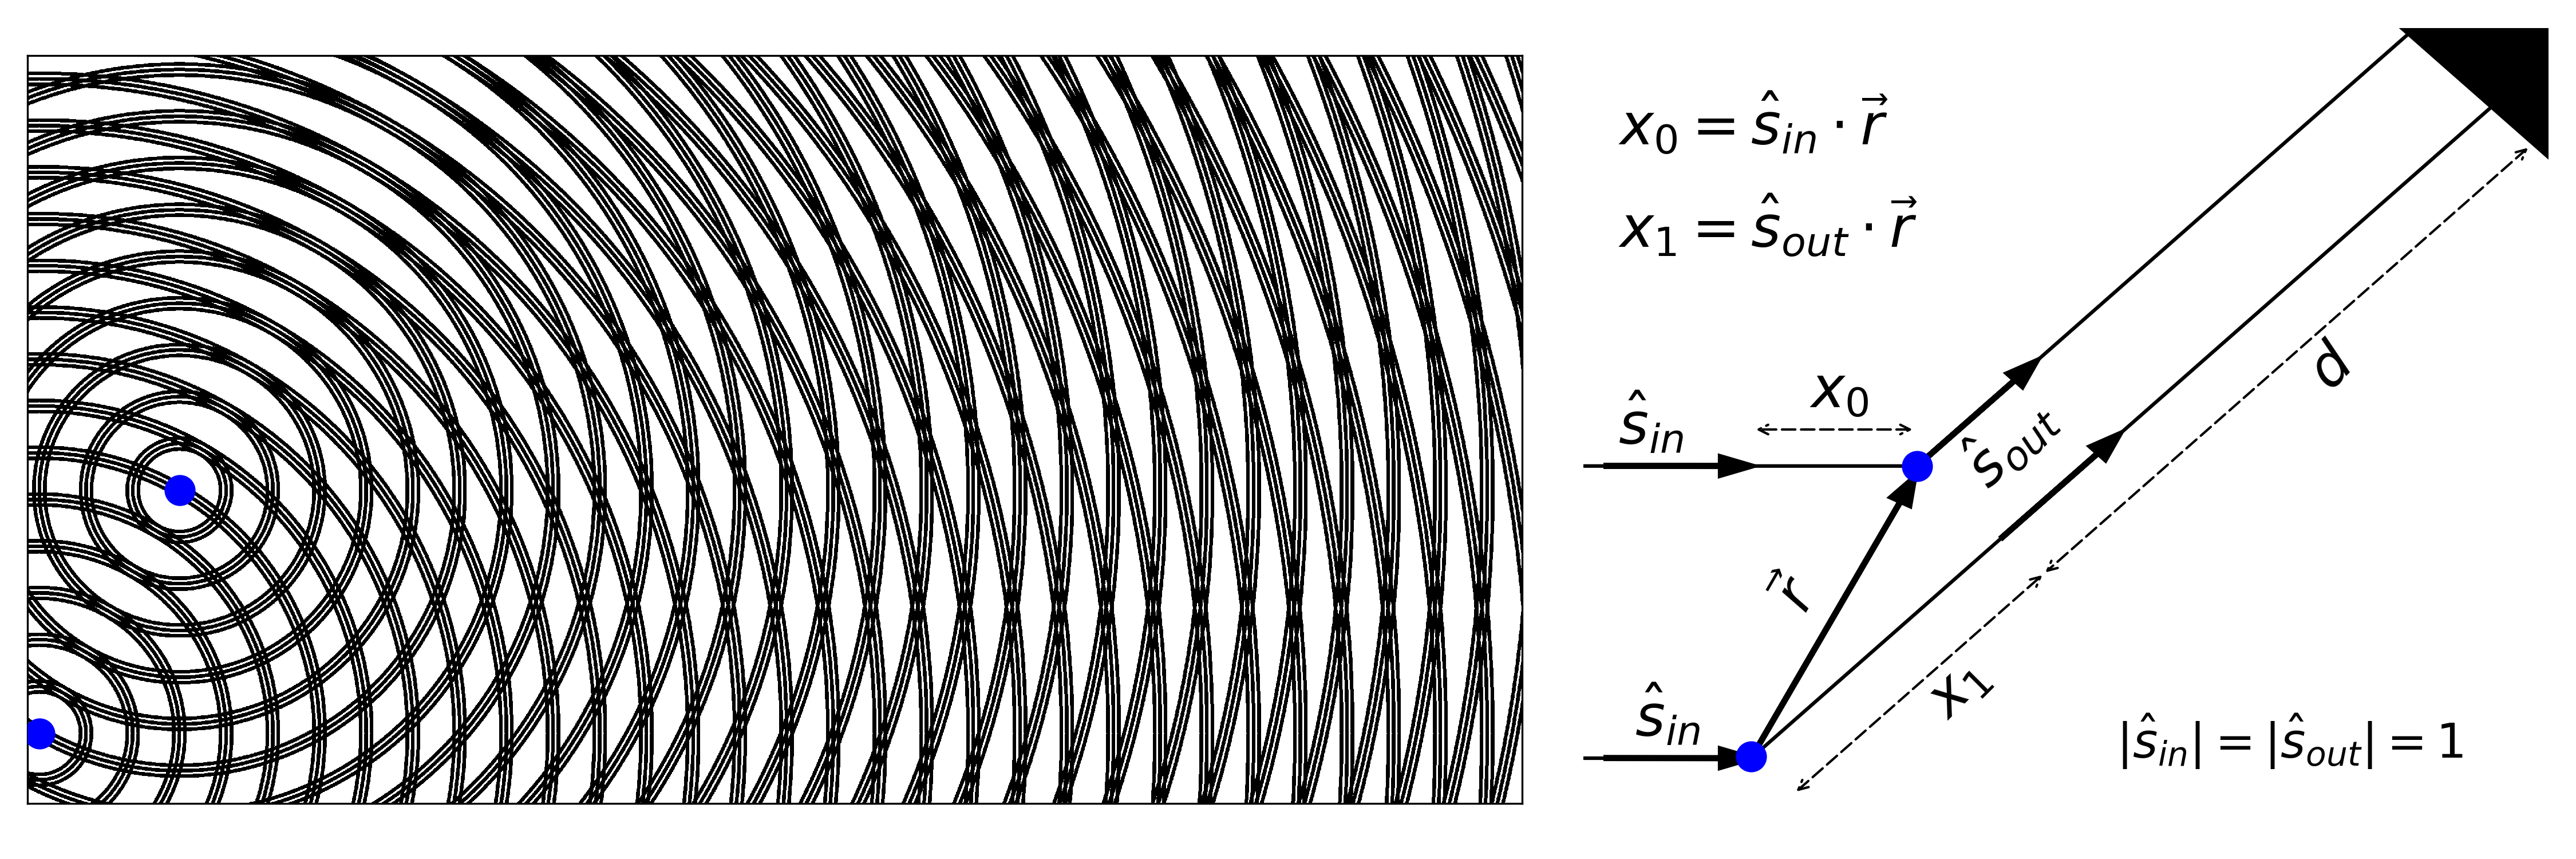
\includegraphics[width=120mm]{InterferenceTwoElectrons3.png}
%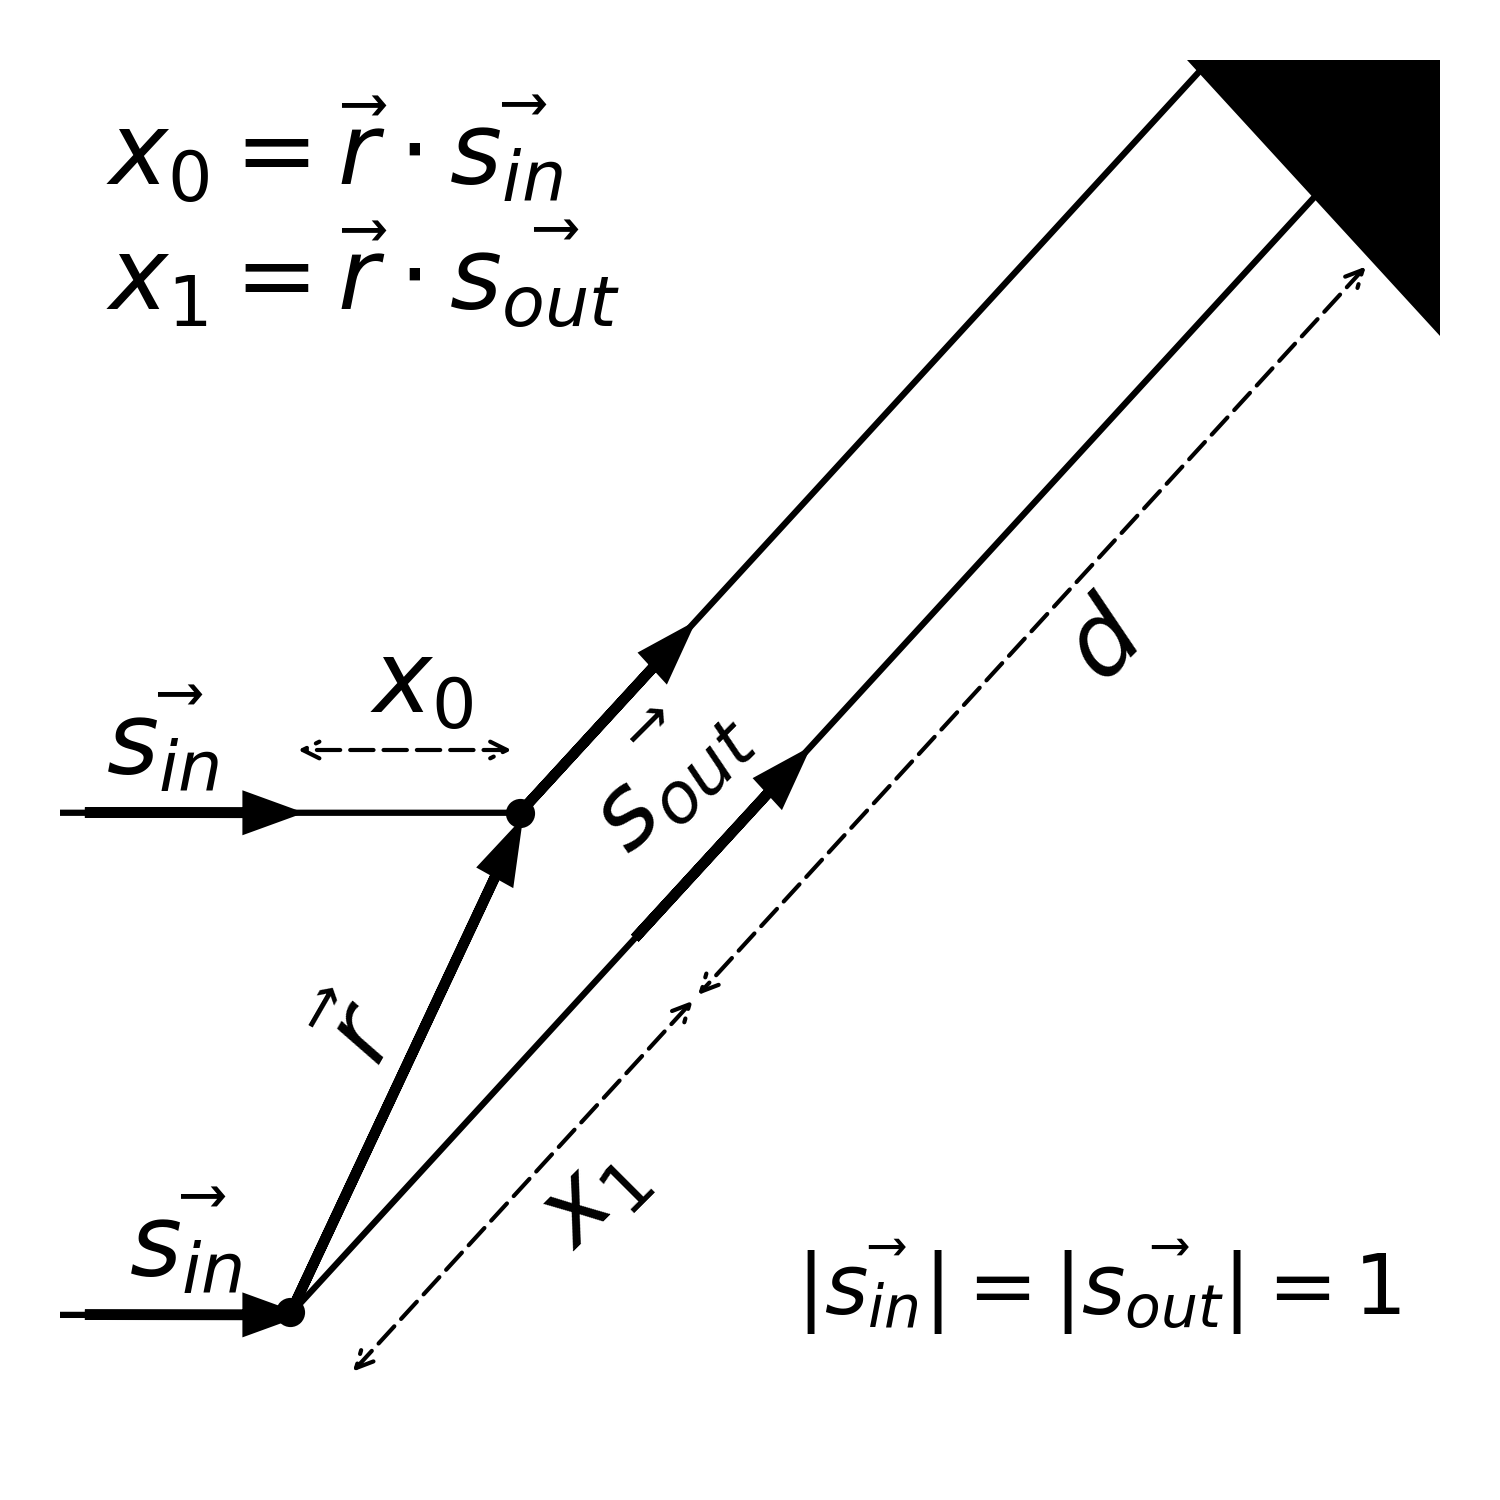
\includegraphics[width=40mm]{blah.png}
\label{fig:Interference}
\caption{Illustration of the scattering from two free-electrons. a) The two blue dots represent two independently scattering free-electrons. The rings represent the maxima of the two scattered waves. One can see the a light-dark band structure appear, characteristic of a interference pattern. b) mathematical description of the path length difference between two waves arriving at point $\vec{d}$. $\hat{s}_{in}$ and $\hat{s}_{out}$ are unit vector pointing in the direction of the incident wave and the out going wave respectively. $\vec{r}$ is a position vector describing the relative distance between the two electrons. }
\end{figure}

If the diffraction pattern is measured at point \(\vec{d}\), far away from the diffracting object itself, both scattered fields have approximately the same field strength since the distance from both electrons to the detector is about equal. In Figure \ref{fig:Interference} this means that  $|\vec{d}+x_1| \approx |\vec{d}|$, and that both $\hat{s}_out$ are parallel. This approximation is called the far-field approximation. The Fresnel number (FN) is used to verify the validity of the far-field approximation.
\begin{equation} 
FN = \frac{o^2}{d\lambda}
\end{equation}
where $o$ is the object size, $d$ the distance from the
object to the detector, and \(\lambda\) the
wavelength of the radiation. The far-field approximation is valid when $FN \ll 1$. All diffraction patterns discussed
in this thesis are taken in the far-field. 

The electric field at point $\vec{d}$ is given by a sum of the individual scattered electric fields:
\begin{equation}
E(\vec{d}) = E_s(\vec{d})+E_s(\vec{d}) e^{\frac{2 \pi\,i\,\Delta x}{\lambda}} 	 
\end{equation}
$\Delta x$ is the optical path difference between the two scattered waves due to the relative difference in position. $\Delta x$ can be determined by summing $x_0$ which is the path difference of the incoming radiation and $x_1$ which is the path difference of the outgoing radiation. Both $x_0$ and $x_1$ can be described using the difference vector $\vec{r}$: 
\begin{equation}
\Delta x = x_0 - x_1 =\hat{s}_{out} \cdot \vec{r}-\hat{ s}_{in}\cdot \vec{r} = (\hat{s}_{out} -\hat{s}_{in} ) \cdot \vec{r} 
\end{equation}

By defining the scattering vector $\vec{S}$
\begin{equation}\label{eq:ScatteringVector}
\vec{S} = \frac{\hat{s}_{out}}{\lambda} - \frac{\hat{s}_{out}}{\lambda}\\ = \vec{s_{out}}-\vec{s_{in}}
\end{equation}
the diffraction pattern of two electrons van be written as:
\begin{equation}
E(\vec{d}) = E_s(\vec{d}) + E_s(\vec{d}) e^{2\,\pi\,  i\,\vec{S}\cdot\vec{r}}
\end{equation}

Implicit in this interpretation is the assumption that the scattered field will not be scattered a second time. This approximation is called the first Born approximation. We assume this to be valid for all objects smaller than a few micrometers.

Important to note is that $\Delta x $ can be at most $|\vec{r}|$, the distance between the two electrons. Abbe demonstrated that in order to resolve two electrons from each other at least two diffraction orders must be captured. This usually means the zeroth and the first order. The first order start where $\Delta x > \lambda/2$. For two electrons closer than half a wavelength apart this will never be the case. This sets a physical limit to the possible details one can resolve using a regular diffraction set-up. One would not be able to use green light ($\lambda = 500\,nm$) to image objects smaller than 250 nm. For structural studies of molecules this means that in order to distinguish single atoms, X-ray radiation is required.

\section{Scattering from multiple electrons}
The framework for describing the scattering of two electrons can easily be extended to N electrons, considering that every electron scatters independently from the others. The electric field can be described as the sum of all the individual scattered fields.
\begin{equation}\label{eq:boehoe}
E(\vec{d}) = E_s(\vec{d}) \sum_{n} e^{2\,\pi\,  i\,\vec{S}\cdot\vec{r_n}}
\end{equation}
where n identifies the individual electrons.

In biological particles the incoming EM radiation is scattered by electrons that are part of atoms, instead of being scattered by free electrons. As we will see, this has a major effect on the scattering process. The scattering potential $\rho(\vec{r},\lambda)$ describes the scattering from a single atom in comparison to the scattering by a free electron. At X-ray wavelengths $\rho(\vec{r},\lambda)$ can be approximated by:

\begin{equation}
\rho(\lambda.\vec{r}) = -r_e (f_1 + i\,f_2)
\end{equation}
Here, $r_e$ is the classical electron radius. $f_2$ is derived from the atomic photoabsorption cross section and is a measure of absorption [booklet]. $f_2$ becomes very relevant close to an absorption edge of the material. $f_1$ describes the scattering power of an atom. It is related to the imaginary part by the Kramers-Kronig dispersion relation [Kramers]. At high photon energies $f_1$ approaches the atomic number of an atom.  

For most elements, the exact value of $f_1$ and $f_2$ have been determined experimentally for a wide range of photon-energies \cite{Henke1990}. Figure \ref{fig:waterwindow} presents the scattering factors of two elements: carbon and oxygen. The energy range from 282-533 eV (4.40 nm - 2.33 nm) is called the water window. In this region, and especially towards the higher energies, oxygen atoms and thus water, are scattering significantly less than the carbon atoms that  make up organic biomolecules. The water window is therefore a good candidate for imaging cells, as the contrast between two of their main constituents, water and biomolecules, is enhanced.

\begin{figure}[h]
\centering 
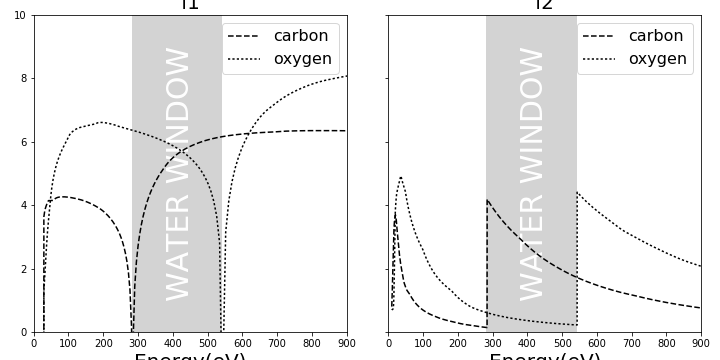
\includegraphics[width=80mm]{waterwindow.png}
\label{fig:waterwindow}
\caption{Atomic scattering factors $f_1$ and $f_2$ of carbon and oxygen, as a function of photon-energy of the X-ray radiation. The region between the absorption K-edge of carbon (282 eV, 4.40 nm) and the K-edge of oxygen (533 eV, 2.33 nm) is called the water window.  The contrast between biomolecules and water is enhanced in this region, especially towards higher photon energies. These wavelengths could be used for imaging living biological particles such as cells or organelles.}
\end{figure}

The scattered field can now be described as follows:

\begin{equation}\label{eq:boehoe2}
E(\vec{d}) = E_s(\vec{d}) \sum_{m} \rho(\lambda,\vec{r}) e^{2\,\pi\,  i\,\vec{S}\cdot\vec{r_m}}
\end{equation}
where $m$ denotes the different atoms.

If all electrons together are assumed to form a continuous electric charge density around the many nuclei that constitute the biological particle, equation \ref{eq:boehoe}  can be written as a continuous function. 

\begin{equation}\label{eq:cont}
E(\vec{d}) = E_s(\vec{d})\int \rho(\vec{r},\lambda) \exp^{-2\pi i \,\vec{S} \cdot \vec{r}}\,d\vec{r}
\end{equation}

We can now introduce the scattering factor $F(\vec{S})$.
\begin{equation}
F\left(\vec{S}\right) = \frac{E(\vec{d})}{E_s(\vec{d})} = F\left(\frac{\vec{d}}{|d|}\right)
\end{equation}
The structure factor is independent of the distance of the detector, it only depends on the angle of measurement. Instead of structure factor, the term molecular transform is often used in the field of crystallography. Throughout this thesis we will use this term as well.

Equation \ref{eq:cont} can be rewritten as:
\begin{equation}\label{eq:diff_equation}
F(\vec{S}) = \int \rho(\vec{r},\lambda) \exp^{-2\pi i \,\vec{S} \cdot \vec{r}}\,d\vec{r}
\end{equation}

This equation is very similar to a well known Fourier transformation $\mathcal{F}( g( t ) )$ []. 

\begin{equation}
 G(\omega) = \int g(t) e^{-2 \pi i \omega\, t}\,dt
\end{equation}

Equation \ref{eq:diff_equation} is very convenient as we now know that, in the far-field, the scattering of a plane wave is proportional to the Fourier transform of the scattering potential evaluated at $\vec{S}$.

We can now also define the inverse relation of \ref{eq:diff_equation}:
\begin{equation}
\rho(\vec{r}) = \mathcal{F}^{-1} ( F(\vec{S}) ) = \frac{1}{2\,\pi}\int F(S) \exp^{2\pi i \,\vec{S} \cdot \vec{r}}\,d\vec{S}
\end{equation}


\section{the Ewald Sphere}

\begin{figure}[h]
	\centering 
	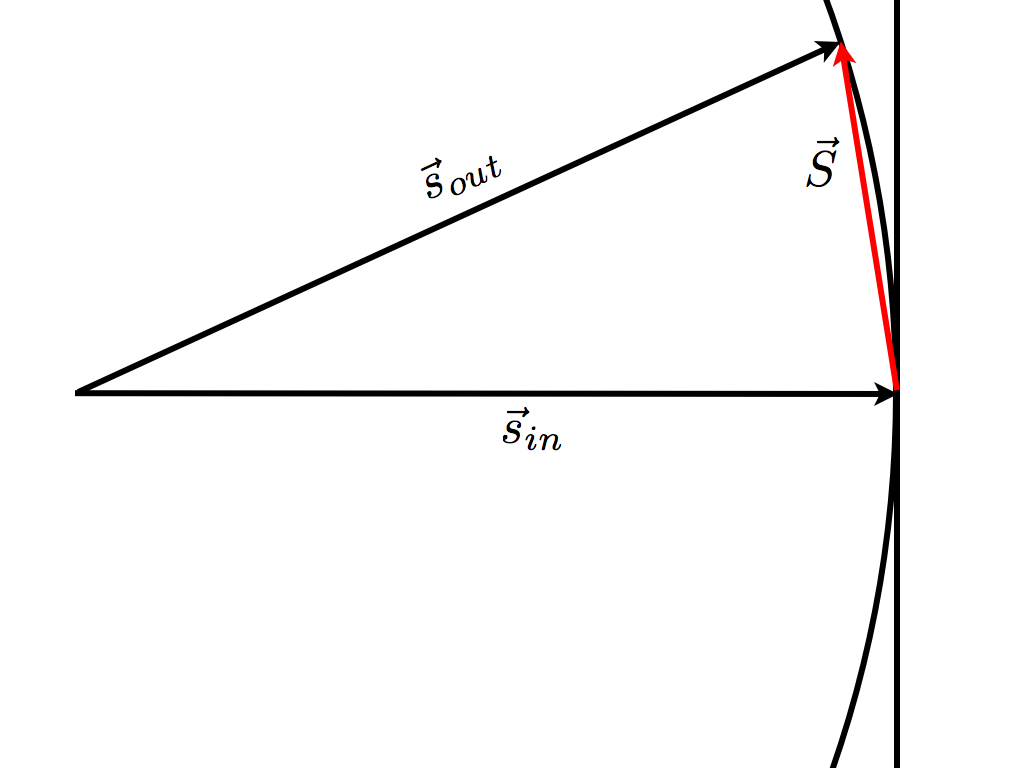
\includegraphics[width=50mm]{ewald_sphere.png}
	\label{fig:EwaldSphere}
	\caption{A schematic of the Ewald sphere. The scattering vector $\vec{S}$ will always reside on the surface of a sphere of length $1/\lambda$, that intersects with the origin of the three-dimensional molecular transform of the object. $\vec{S} = \vec{s}_{in} - \vec{s}_{out}$. $\vec{s}_{in}$ is constant and is determined by the direction of the incoming radiation. $\vec{s}_{out}$ has a constant length, but varies in direction with scattering angle $\theta$. }
\end{figure}

The molecular transform $F(\vec{S})$ of a three-dimensional object is also three-dimensional. A diffraction pattern, however, is not. To understand this, we have to evaluate $\vec{S}$ more carefully. 

In a diffraction experiment $\vec{S} = \vec{s}_{out} -\vec{s}_{in}$ (see equation \ref{eq:ScatteringVector},). $\vec{s}_{in}$ is constant, and is determined by the propagation direction of the incoming EM field. $\vec{s}_{out}$ has a fixed length ($1/\lambda$), and points in the direction of the scattered field ($\theta$). The scattering vector $\vec{S}$ is therefore limited to reside on the surface of a sphere of radius $1/\lambda$. This sphere is called the Ewald sphere [] (see Figure \ref{fig:EwaldSphere}). 


The Ewald sphere intersects the $F(S)$ through its center $F(0)$. At small scattering angles the curved Ewald sphere can considered to be flat. This means that a diffraction pattern can be approximated as slice through the center of the molecular transform.  This relation will prove itself to be very useful.

\section{Properties of the Fourier transform}
There is a large mathematical field describing the properties of Fourier transformations. A few of these relations are very useful to this thesis.
\begin{enumerate}

\item Linearity\\
	For any complex number $a$, if $h(t) = a g(t)$, then $H(\omega) = a \, G(\omega)$

\item Scaling\\
	For any non-zero real number $a$, if $h(t) = g(a t)$, then $H(\omega) = \frac{1}{|a|} G\left(\frac{\omega}{a}\right)$

\item Translation\\
	For any real number $t_0$, if $h(t) = a g(t+\Delta t)$, then $H(\omega) = e^{2\pi\,i\,\Delta t \omega} G(\omega)$. The factor $e^{2 \pi i \Delta t \omega}$ is called a 'phase-ramp'.

\item Convolution\\
The Convolution theorem states that a multiplication in Fourier space is a convolution in object space (real space) and vice versa.
\begin{equation}
f(t) * g(t) = \int f(\tau)g(t-\tau)\,d\tau = \mathcal{F}^{-1} \left( \mathcal{F}(f(t))\,\mathcal{F}(g(t))\right)
\end{equation}

\item {Projection Approximation}\\
The projection slice theorem states that the Fourier transform of the projection of an three-dimensional function g(t) onto an two-dimensional plane is equal to an two-dimensional slice through the origin of the three-dimensional Fourier transform of the function g(t)
which is parallel to the projection plane. At small scattering angles, a diffraction pattern is a slice through the center of the three-dimensional Fourier transform. In this case the results of equation can be interpreted as a projection of the scattering potential. 

\item {Discrete Fourier Transform}\\
In practice we are dealing with a signals that are not continuous, but discrete. Most signal recording is done digitally, and to be able to do numerical computations on the signal, it has to be digitized as well. For discrete signal the discrete Fourier transform (DFT) and the inverse discrete Fourier transform (IDFT) can be used.

\begin{equation}
DFT( g( T_{k,l,m} ) ) = G( \Omega_{k,l,m} ) = \sum_{k=1}^{K} \sum_{l=1}^{L} \sum_{m=1}^{M} g( T_{k,l,m} ) e^{-2 \pi i \Omega_{k,l,m} \cdot T_{k,l,m}}
\end{equation}

\begin{equation}
IDFT( G( \Omega_{k,l,m} ) ) = g ( T_{i,j,k} ) = \frac{1}{{K L M}} \sum_{k=1}^{K} \sum_{l=1}^{L}\sum_{m=1}^{M} G( \Omega_{k,l,m} ) e^{2 \pi i \Omega_{k,l,m} \cdot T_{k,l,m} }
\end{equation}

where $K$,$L$ and $M$ are the number of 3D pixels (voxels) in each dimensions. $T_{k,l,m}$ and $\Omega_{k,l,m}$ are the discretized version of $t$ and $\omega$. 

\end{enumerate}

\section{Radiation Damage}
The scattering power of an object is proportional to its volume, and thus varies with the 3rd power of its size. The smaller an object is, the less scattering occurs. To compensate for this loss in scattered signal, the required dose for imaging increases. Practically this means that a dose in excess of 100 MGy is required to record an interpretable signal from a living cell. To put this in perspective, a dose of 2000 Gy is already enough to kill an organism that lives on earth. This means that the amount of energy deposited into the system through photoabsorption is not negligible. The main process of photoabsorption at soft-X-ray wavelengths is  photoionisation. Many process follow the ionization event, of which non-radiative Auger decay can lead to significant radiation damage throughout the material. The relation between the required dose of radiation versus the maximum tolerable dose of radiation posed a physical limit to the obtained resolution for imaging single biomolecules [Howell].

\section{Diffract-before-destroy}
An elegant solution to the problem of radiation damage came from the realization that elastic scattering occurs on a  time scale shorter than the damage processes manifest themselves structurally. This principle is of diffract-before-destroy, suggested in 2000 by Neutze \textit{et al.} \cite{Neutze2000}, was experimentally demonstrated on a silicon-nitrate sample \cite{Chapman2009}. This experiment used the ultra short and extremely bright pulses from the first x-ray free-electron laser to outrun key damage processes \cite{Chapman2000}. Although the pulse literally obliterated the sample, enough structural information was captured to retrieve the original structure. A single XFEL pulse has a power densities of $10^{16} W/cm^2$, and can be between 1-100 fs long. This facilitates the imaging of single particles at room temperature.

Diffract-before-destroy has been further validated by a wide variety of experiments \cite{Seibert2009,Seibert2010}. Serial femtosecond crystallography (SFX) showed that with this principle at least three orders of magnitude higher radiation doses are tolerated compared to regular crystallography, enabling the imaging of much smaller crystals []. The imaging of single particle has been shown feasible in 2D for a wide variety of biological particles, ranging from \textit{living} cells (\textbf{Paper I}) to cell organelles (\textbf{Paper VXIII}) to  40 nm viruses (\textbf{Paper XIV}). \textbf{Paper XVII} shows the experimental feasibility of using many 2D images to construct a 3D model of a giant virus.

The field is very close to measuring the first 2D diffraction patterns of single proteins. For simulated data it has been shown that such patterns can be used to recover the 3D shape of proteins, even though the number of scattered photons might be as low a 1000 photons per frame. The ultra short pulses also allow for the studying of the dynamics of such systems, either by separating the images from different naturally occurring conformational states, or by identifying structural changes subsequent to an external trigger []. In the more distant future these structural changes might be tracked inside living cells. 
 
    \chapter{Pulse Generation by XFEL}
Free-electron lasers (XFELs), invented by J. Madey and demonstrated experimentally in the 1970s, can generate multi gigawatt and femtosecond (fs) x-ray radiation. Compared to fourth generation synchrotrons, this is a ten billion-time increase in brightness. Typically an XFEL consists of three sections: i) the electron gun, ii) a linear accelerator, and iii) an undulator. The x-ray radiation is generated in the undulator. Figure 1 shows a schematic of the XFEL at the Linear Accelerator Coherent Light Source (LCLS) at Stanford. This chapter will describe the operating of the LCLS in specific. Other XFELs might use different hardware, but the fundamental principles that drive an XFEL will be very similar. Please note that the words bunch and pulse are used to discriminate between a collection of electrons and radiation respectively.

\begin{figure}[h]\label{fig:LCLS}
\centering
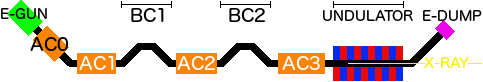
\includegraphics[width=100mm]{Chapter_03_LCLSSchematic.png}
\caption{Schematic of LCLS. Electron bunches are created by the electron gun (E-gun). The bunches are consecutively accellerated by linear accelerators (AC0-3) and compressed by bunchcompressors (BC0-1). After the final acceleration the bunch is guided into the undulator, where an x-ray pulse is generated. After the undulator the x-ray pulse continuous to the beamline, and the electron bunch is dumped (E-dump).}
\end{figure}

In the electron gun, a copper plate is irradiated by a powerful ultraviolet laser pulse, which releases a bunch of electrons. At this moment the electron bunch is a few picoseconds long and has a peak current less than 100 A. As shown in figure \ref{fig:AC}a, the energy spread within the bunch is minimal at this point. The electron bunch is directly accelerated to 99.7\% of the speed of light, using a standing wave in a RF cavity (AC0). Due to cooling reasons in AC0 the LCLS produces electron pulses at maximally 120 Hz. 

\section{Klystron}

Consecutively the bunches are guided in a long series of accellerating units named klystrons. See AC1-3 in figure \ref{fig:LCLS}, and for more detail figure\ref{fig:AC})d. In essence a klystron is a cylinder on which an strong MHz alternating current is applied. The AC current induces a EM field in the MHz range (RF), similar to the way radiowaves are produced in an antenna. Due to the spacing between irises the relative phase velocity of the wave is matched to the speed of the electrons, thus through the Lorentz force longitunal acceleration can be achieved throughout the whole klystron. In the center of the cavity the magnetic field is zero, the acceleration is therefore proportional to the strength of the electric field. Each klystron can maximally add 30 MW/m of energy to the electron bunch. Under higher currents the klystron will tear itself apart. In order to reach 15 GeV electron bunches at least 500 m of klystrons are needed. In reality the accelerating unit of LCLS are 889 m long. Often accelerators do not operate at the point of maximum acceleration, since one wants to introduce a negative energy gradient along the particle bunch, that can later be utilized for bunch compression. This acceleration method is called off-crest acceleration, and is visualized in figure  \ref{fig:AC} b and d. A negative energy gradient means that the electrons located at the front of the bunch have a slightly lower energy compered to electrons the electrons are located at the rear of the bunch.

\begin{figure}[h]\label{fig:AC}
\centering
\includegraphics[width=100mm]{Chapter_03_Acceleration_v2.png}
\caption{Schematic of acceleration and bunch compression at LCLS. a-c) change of bunch shape throughout the accelerator. d) illustration of the off-crest accelleration principle. a) shows that  This creates an energy chirp. e) schematic of a single klystron. f) schematic of a chicane. The green and red blocks are magnetic dipoles that deflect the electron bunch in opposite direction. The path of high energy electrons diverges less than lower energy electrons. If the bunch has a negative energy chirp, this results in bunch compression.}
\end{figure}

\section{Bunch Compression}
Short and compact bunches are essential for the functioning of an XFEL. One of the main bunch-compression devices are chicanes. Chicanes consist of four magnetic dipoles that diverge the high energy part of the bunch less than the low energy part (see figure \ref{fig:AC} ). Due to the negative energy gradient it thus reduces the temporal spread of the bunch. After the final compression the electron bunch is ~40fs long, has a peak current of 4.3 kA, and travels at 99.999\% of the speed of light. The relastivistic $\gamma \sim 2000$. Creating these type of bunches is a noteworthy technical achievement, 

\section{Undulator}
\subsection{Monochromatic X-ray radiation}
The undulator is the heart of an XFEL. It is a periodic arrangement of magnets with alternating poles. The magnetic field of a periodic magnetic structure can be written as:
\begin{equation}\vec{B}(z) = B_0\cos{(\frac{2\pi}{\lambda_u}z)}\hat{\mathbf{y}}\label{eq:bz}\end{equation}
$B_0$ is the magnetic field, $\lambda_u$ is the wavelength of an undulator period.
Due to the magnetic field the moving bunch of electrons experience a Lorentz force, causing it to oscillate in the transverse direction (x). The movement can be described by the following equation. 
%\begin{equation}\vec{F} = e(\vec{v}\times\vec{B})\end{equation}
\begin{equation}v_x = \frac{-e\,B_0\,\lambda_u}{2\pi\,m_e\gamma} \sin{(\frac{2\pi}{\lambda_u}z)} = \frac{K c}{\gamma} \sin{(k_uz)}\label{eq:vx}\end{equation}
Usually the non-dimensional parameter K is written as:
\[K =  \frac{-e\,B_0\,\lambda_u}{2\pi\,m_e \, c}  \approx 0.9337 B_0 \lambda_u\]
where the magnetic field is measured in Tesla and the undulator period in centimeters.

Preserving momentum the oscillating electrons emit radiation ($\lambda_s$). As described in chapter 1, interference effects will occur between the emitted waves from the different charges (remember the electrons come in a bunch which has a size). The essence of this interference phenomenon lies in the longer route taken  by the oscillating electrons compared to the radiation, which causes an OPD between the radiation emitted by electrons one undulator period apart. If the OPD between the electrons and the radiation is equal to and integer of $\lambda_s$, the emitted waves will add coherently. Radiation with other wavelengths will interfere destructively. The longer an undulator the more pronounced the selection of specific wavelengths. Equation \ref{eq:res} describes this so-called resonance condition.%, as shown in figure 3b.
\begin{equation}c\frac{\lambda_u}{<v_z>} -\lambda_u\, \cos{(\theta)} = n \lambda_s \label{eq:res}\end{equation}
To predict at which wavelength this happens we need to find the average longitudinal velocity $v_z$. As the total speed $v$ of the electrons is not affected by the Lorentz force, $v_z = \sqrt{ {v}^2-{v_x}^2}$\footnote{Using Pythagoras' theorem}. Using Equation \ref{eq:vx} for $v_x$ and $\gamma^2 \equiv (1-\frac{v^2}{c^2})^{-1}$, we can write $v_z$ as: 
\[ v_z = \sqrt{c^2(1-\frac{1}{\gamma^2})-\frac{K^2 c^2}{\gamma^2}\sin^2(k_u\,z)} = c \sqrt{1-\frac{1}{\gamma^2}(1-K^2\sin^2(k_u\,z))}\]
Using the mathematical identity $\frac{1}{\pi}\int_{0}^{\pi} \sin^2( x ) \, dx =\frac{1}{2} $, integrating of half a undulater period gives the average velocity $<v_z>$.
\[<v_z> = c\sqrt{1-\frac{1}{\gamma^2}(1-\frac{K^2}{2})}\]
${\gamma} \gg 1$, thus we can expand the root $\sqrt{1+x} = 1+\frac{1}{2}x-\frac{1}{8}x^2+ ...$ (first order Taylor expansion).
\[<v_z> \approx c(1-\frac{1}{2\gamma^2}(1+\frac{K^2}{2}) )\]
If we now assume that we only observe the radiation in the forward direction, we can expand $\cos{(\theta)} = 1-\frac{\theta^2}{2}$. 
Equation \ref{eq:res} can thus be written as:
\[ n \lambda_s = \lambda_u[\frac{1}{1-\frac{1}{2 \gamma^2}(1+\frac{K^2}{2})} - (1-\frac{\theta^2}{2})]\]
The geometrical series $\frac{1}{1-x} = 1+x+x^2+...$ allows us to obtain the well known undulator equation.
\begin{equation} n \lambda_s = \frac{\lambda_u}{2 \gamma^2}(1+\frac{K^2}{2}+(\gamma\theta)^2)\end{equation} 

This formula can be explained by two relativistic effects. For an observer it is the electron bunch that is moving close to the speed of light. In the electron bunch's frame of reference however it is the undulator that is moving very fast. Fast objects are length contracted, thus the electrons observes a undulator period of $\frac{\lambda_u}{\gamma}$, which makes it emit radiation with $\lambda$ around $\frac{c\lambda_u}{\gamma}$. The radiation is relativistically contracted when observed in the laboratory's frame of reference (relativistic doppler effect), adding the second gamma term. The size of relativistic doppler effect is dependent on the angle of observation relative to the direction of motion. 

The final wavelength of the emitted light is thus dependent on the energy of the electrons ($v$), the magnetic field in the undulator ($B$), and the angle of observation ($\theta$). Control over these variables makes the selection of a specific wavelength possible. LCLS can produce X-ray radiation in the range of 400 eV -10 keV. 


%\subsection{Direction of Emission}
\subsection{SASE}
So far the emitted radiation is monochromatic, but not temporally coherent. This means the total emitted power is proportional to the number of the electrons in the bunch ($N_e$). If all emitted radiation would emit in phase, the total irradiated power would be proportional to ${N_e}^2$. Pellegrini and others realized that for short pulses, and long undulators, temporal coherence could by achieved by a process called Self Amplified Stimulated Emission (SASE). SASE exploit the slight non-uniformities in the electron bunch, that cause radiation with a certain phase to be slightly more prevalent than others. The Coulombic force exerted by the electric field of this radiation will start grouping electrons at its nodes (See figure 2). Electrons are accelerated when the electric field is positive, and decelerated when negative, causing the so-called microbunches to appear. This process forms a positive feedback loop, causing a exponential increase in radiation power. The  exponential  growth  cannot  continue  indefinitely, and  the  power  must  saturate  at  a  certain  level. The SASE process ultimately saturates when either the electrons loose so much energy the resonance condition is not met anymore, or when the energy of the radiation surpasses that of the electron bunch. In the latter case the EM wave will start to transfer energy to the electron bunch instead\footnote{This phenomenon is similar to inverse Compton scattering, in which electrons absorb energy from the radiation field.}.

The high power density within the pulse means that there are more than one photon in the volume of a $\lambda^3$. Which means that so far diffraction patterns come from single photons interfering with themselves []. Interference between more than one photon might be different. For example there might be special interactions between photons. 






    \chapter{Substrate-free sample delivery}
In FXI everything that is illuminated by the X-ray pulse is sample. In the case of weakly scattering single particles scattering from any substrate around the might drown the signal from the particle itself. Aerosol injection removes this clutter and assures that the sample is clearly isolated from its surroundings, and this, as we see in a later chapter 6, is important for image recovery.

An aerosol injector produces small droplets of particles dissolved in a volatile buffer. The buffer evaporates under the reduced pressure inside the experimental chamber, ideally leaving behind only the particle. There are two main types of nozzles that can be used to produce small drops: the Gas Dynamic Virtual Nozzle, and electro spray ionisation (ESI).

\begin{figure}[h]\label{fig:drop_formation}
\centering 
\includegraphics[width=120mm]{Chapter_04_GDVNEvaporation.png}
\includegraphics[width=120mm]{ESI_drop_evaporation_explosion.png}

\caption{Experimental geometry, including different sample delivery system. From the bottom left the x-rays pulses enter the chamber. The experimentalist can now select a sample delivery system. Shown are an aerosol sample delivery system, liquid jet injection system, and two types of substrate bound sample delivery systems. If the beam intersect the sample (and/or substrate) a diffraction pattern is recorded on two sets of detectors, placed at different distances from the interaction region.}
\end{figure}




\subsection{Gas Dynamic Virtual Nozzle}

If the coaxial flow of gas creates a jet with a diameter smaller than then a characteristic $d_j$ the surface tension in the liquid will cause the jet to break up into a mist of small droplets. $d_j$ can be estimated on the basis of energy conservation, and is a function of the effective pressure drop $\Delta P$. It is assumed that all energy is transformed to kinetic energy \cite{Acero2013}.
\begin{equation}
d_j^{(GDVN)} = 2 \sqrt{Q \cdot \left(\frac{\rho}{2 \pi^2 \Delta P}\right)^{1/2}}
\end{equation}    
$Q$ denotes the flow rate and $\rho$ is the density of the liquid. The final drop diameter $d_d$ can be related to the jet diameter using the ratio $d_d / d_j \approx 1.9$, which is the classical Rayleigh breakup []. Empirically this assumption has been shown to work well for low-viscosity media such as water. The GDVN can create droplets in the size range of 400 nm - 2000 nm. Sample consumption is in the range of ul/min.

\subsection{Aerodynamic Lens Stack}
After the droplets formed, they start to evaporate in the reduced pressure environment, leaving only the non-volatile particles in the 'drop'. The aerosolised particles are guided into an aerodynamic lens stack (see figure ). This is a series of cylindrical cavities, connected by co-aligned orifices, that collimate the droplets into a narrow beam of particles [].

\begin{figure}[h]\label{fig:skimmer_aerolens}
\centering 
\includegraphics[width=120mm]{Chapter_04_SkimmerAerodynamicLens.png}
\caption{Experimental geometry, including different sample delivery system. From the bottom left the x-rays pulses enter the chamber. The experimentalist can now select a sample delivery system. Shown are an aerosol sample delivery system, liquid jet injection system, and two types of substrate bound sample delivery systems. If the beam intersect the sample (and/or substrate) a diffraction pattern is recorded on two sets of detectors, placed at different distances from the interaction region.}
\end{figure}

For robust particles, which are large compared to the drop size, this type of sample injection has proven to be very successful. This sample injection method made it possible to measure the diffraction patterns from isolated single particles at high signal-to-noise ratios at very high repetition rates. Up to 80\% hit rates have been recorded with a 120 Hz repetition rates at the LCLS \cite{Hantke2013}. The results discussed in this thesis come from datasets that were generated using the GVDN injection method.

For many samples aerosol injection is not disruptive. Molecular dynamics simulation have shown that the conformation of proteins is conserved up till the moment that the last structural water evaporates[]. For the cyanobacterial cells described in this paper it has been shown that the shape and the autofluorescence properties of the cell membranes of the injected cells remain unchanged [PAPER I]. This is not quite unexpected. Aerosols of cyanobacteria can be carried for long distances, and metabolically active cells have been detected at altitudes of 20-70 km where atmospheric pressure drops to below a millibar []. Other sample cell lines such as \textit{E. coli} and brewers yeast, and many types of viruses have been shown to be viable after injection. Nevertheless, not all sample types may be amenable to aerosol sample injection, and samples should be tested prior to experiments.  

\subsection{Electro Spray Ionisation}
Over the last years it became apparent that GDVN sample injection does have its limitations. If the particle becomes small compared to the drop size, wide size distributions of otherwise uniformly sized particles were measured [Daurer, Hantke]. These observations might be explained by a combination of an incomplete evaporation process, and the build up of a significant shell of debris, originating from impurities present in the solution, around the particle. To purify the measured sample, smaller drops had to be generated. A common aerosolisation technique used in mass spectrometry called electro spray ionisation (ESI) is known to be able to produce small droplets.

ESI nozzles produce droplets through a similar droplet formation process as occurs in the GDVN. The difference lies in the process that drives jet acceleration. In ESI the jet is accelerated by an externally applied electrostatic potential. In the capillary the solvent (volatile buffer) is mixed with negatively charged ions. By applying an external field these ions are accelerated, accelerating the entire jet. The accelerated jet will ultimately break into small drops similar to what occurs in a GDVN. The characteristic $d_j^{ESI}$ can be described as a function of the surface tension $\sigma$, vacuum permittivity $\varepsilon_0$, electrical conductivity $C$, as well as the flow rate and the density of the liquid.
\begin{equation}
d_j^{(ESI)} \approx 2 \sqrt{Q \cdot \left(\frac{\rho \varepsilon_0}{\sigma C}\right)^{1/3}}
\end{equation}

After the process of evaporation initiates, an electric potential further builds up in the drops, eventually leading to a Coulomb explosion of the drops [Cole]. Cycles of evarporation and explosion leads to smaller and smaller drops. Initial experiments showed that drops of mono disperse droplets of size 150-200 nm can be generated with ESI. ESI can also be combined with an aerodynamic lens stack. 

The transfer of ESI to FXI is a considerable achievement that will allow the field to move forward to image smaller particles such as proteins. This would not have been possible using the GDVN aerosolisation. ESI has been shown to also function under lower flowrates, reducing sample consumption to 10 nl/min []. This sample consumption rate is advantageous for samples that are only available in small quantities. 

\subsection{Drop-on-demand}
The combination of ESI and a quadrupole with an ion trap for storage allows for a pulsed delivery system that can be tuned to match the repetition rate of the XFEL. This is generally referred to as drop-on-demand. This would reduce the sample consumption even further. Moreover the ion trap can also be utilized for sample selection prior to injection of sample into the x-ray pulse. This is important for single proteins as they scatter very little signal, which makes it very difficult to separate the diffraction patterns from the particle-of-interest and those diffraction patterns obtained from contaminating particles or other noise. 


    \chapter{Data recording}
As we have learned in chapter 2, a diffraction pattern is the Fourier transform of the scattering potential, sampled at the Ewald sphere ($F{\vec{S}}$). The scattering potential is determined by the structure of the object which is sampled. If a diffraction pattern measures the low scattering angles, the curved Ewald sphere might be approximated as being flat. This chapter will describe the essentials of the process of actually measuring the diffracted signal.

The value of $F{\vec{S}}$ is complex. The complex amplitude corresponds to the amplitude of the measured wave, and the complex argument corresponds to the phase shift of the wave.
Currently no device exists capable of measuring the phase of x-rays directly, as it changes in the attosecond range. The amplitude of the EM wave can be determined through an intensity measurement. 

\begin{equation}
I(\vec{S}) = |F(\vec{S})|^2
\end{equation}

In the experiments described in this thesis we used a so-called pnCCD detector to determine the $I(\vec{S})$. A pnCCD is a 2D array of pixels of size $p$. Each pixel registers the intensity of the EM wave at that location by converting the energy present in the EM wave into an electrical current, using a physical process called the photo-electric effect (a type of photoabsorption). 

$F(\vec{S})$ is independent from detector distance $d$, while a diffraction pattern is not. The relative scaling factor between the two is $\frac{1}{\lambda\,d}$. This means that the area covered by a pixel of size $p$ on the detector covers an area of size $q = \frac{p}{\lambda \, d}$ of the Ewald sphere (given the small angle approximation holds). 


Using the scaling relation between $F(\vec{S})$ sampled at the Ewald sphere, and the measured diffraction pattern at the detector, we can derive that pixel $P$ on the detector corresponds to pixel $\vec{Q} = \frac{\vec{P}}{\lambda\,d}$ on the Ewald sphere. 

Since $F(\vec{S})$ is measured at discrete locations, we have to use the discrete Fourier transform (DFT), and its inverse, to describe the relation between the measured diffraction pattern and the scattering potential. From now on we will use $F(\vec{Q})$ to describe $F(\vec{S})$ measured at discrete positions. 

The use of the DFT implies that the scattering potential is also discretized. The pixel size in real space (scattering potential space) $r$ is the inverse of the size of the detector in Fourier space ($D$). $D = n\,q$, where $n$ in the number of pixels on the detector, $q$ is the size of a pixel on the Ewald sphere. $q$ is the scaled version of a detectro pixel $q = \frac{p}{\lambda d}$. This makes $r$
\begin{equation}
r = \frac{\lambda\,d}{n\,p}
\end{equation}
Here $\lambda$ is the wavelength of the radiation, $d$ the detector distance, and $p$ is the size of a detector pixel.

%In a measurement the energy of a EM wave appears quantized, which means that one will always measure an integer number of the basic quantum of radiation: photons. The energy of a photon is related to its wavelength. The quantisation the measured intensity also has as an effect on the statistics, as they ar

\section{Missing Data}
The geometry of the detectors used in the experiments described in this thesis consist of two moveable halves (38.4 mm by 76.8 mm), with a dead area of at least 0.8 mm in between both halves (see figure \ref{fig:experimental_geometry}). In the center of the
detector a hole is created to let the high-intensity direct beam through (each detector halve misses a semicircle). For both the dead area, and the central hole no intensity information present. As a result the diffraction pattern is incomplete. 

In some experiments two pairs of detectors are used, in which one pair located closer to the sample (see figure \ref{fig:experimental_geometry}). The back detector is closed, and the front detector is opened such that is does not shadow the back detector.
 
\section{Saturation}
Besides missing data due to the detector geometry, detector saturation might also lead to missing information. Each pixel on the detector can maximally hold a certain amount of electrical charge. If more charge is present in the pixel, the excess charge will overflows to neighbouring pixels, making it impossible to accurately use the original and the
affected pixels. If the amount of charge is very high, saturation might even damage the detector itself. Saturation usually occurs in the center of the detector, because these regions are typically the most intense regions of a diffraction pattern. 





    \chapter{Phase Retrieval}
The problem of missing phase information is well known and is called the phase problem. There are many ways to overcome it: for example in crystallography homology modelling or the anomalous scattering of heavy atoms is exploited to retrieve phases. Holography uses the interference between two wave fields to obtain the phases. Ptychography uses the precisely known overlap and high redundancy between many exposures to solve the phase problem. In CXI the scattered field gets oversampled, which means that phases can under certain conditions be retrieved from the intensity pattern itself. The next sections will describe oversampling in more detail, explain how phases can be retrieved from an oversampled signal using an iterative phase retrieval method, and finally how phase retrieval can be validated. 

\section{Oversampling} 
In 1952 Sayre noticed that the Bragg peaks sample the molecular transform $\mathcal{F}(H)$ at the critical sampling rate ($S_C$)\cite{Sayre1952a} (See Shannon \cite{Shannon1949a}). This means that knowing the phases belonging to the Bragg peaks is just enough to back-calculate the structure of the measured object. Single particle imaging is free from the crystal lattice, and isolated Bragg peaks give way to a continuous diffraction pattern. By choosing the detector distance appropriately such that individual pixels cover a small enough angle, we can sample the molecular transform more finely than the critical sampling rate. This sampling condition is called oversampling. Figure \ref{fig:sampling} illustrates both cases of sampling. 

\begin{figure}[h]
	\centering 
		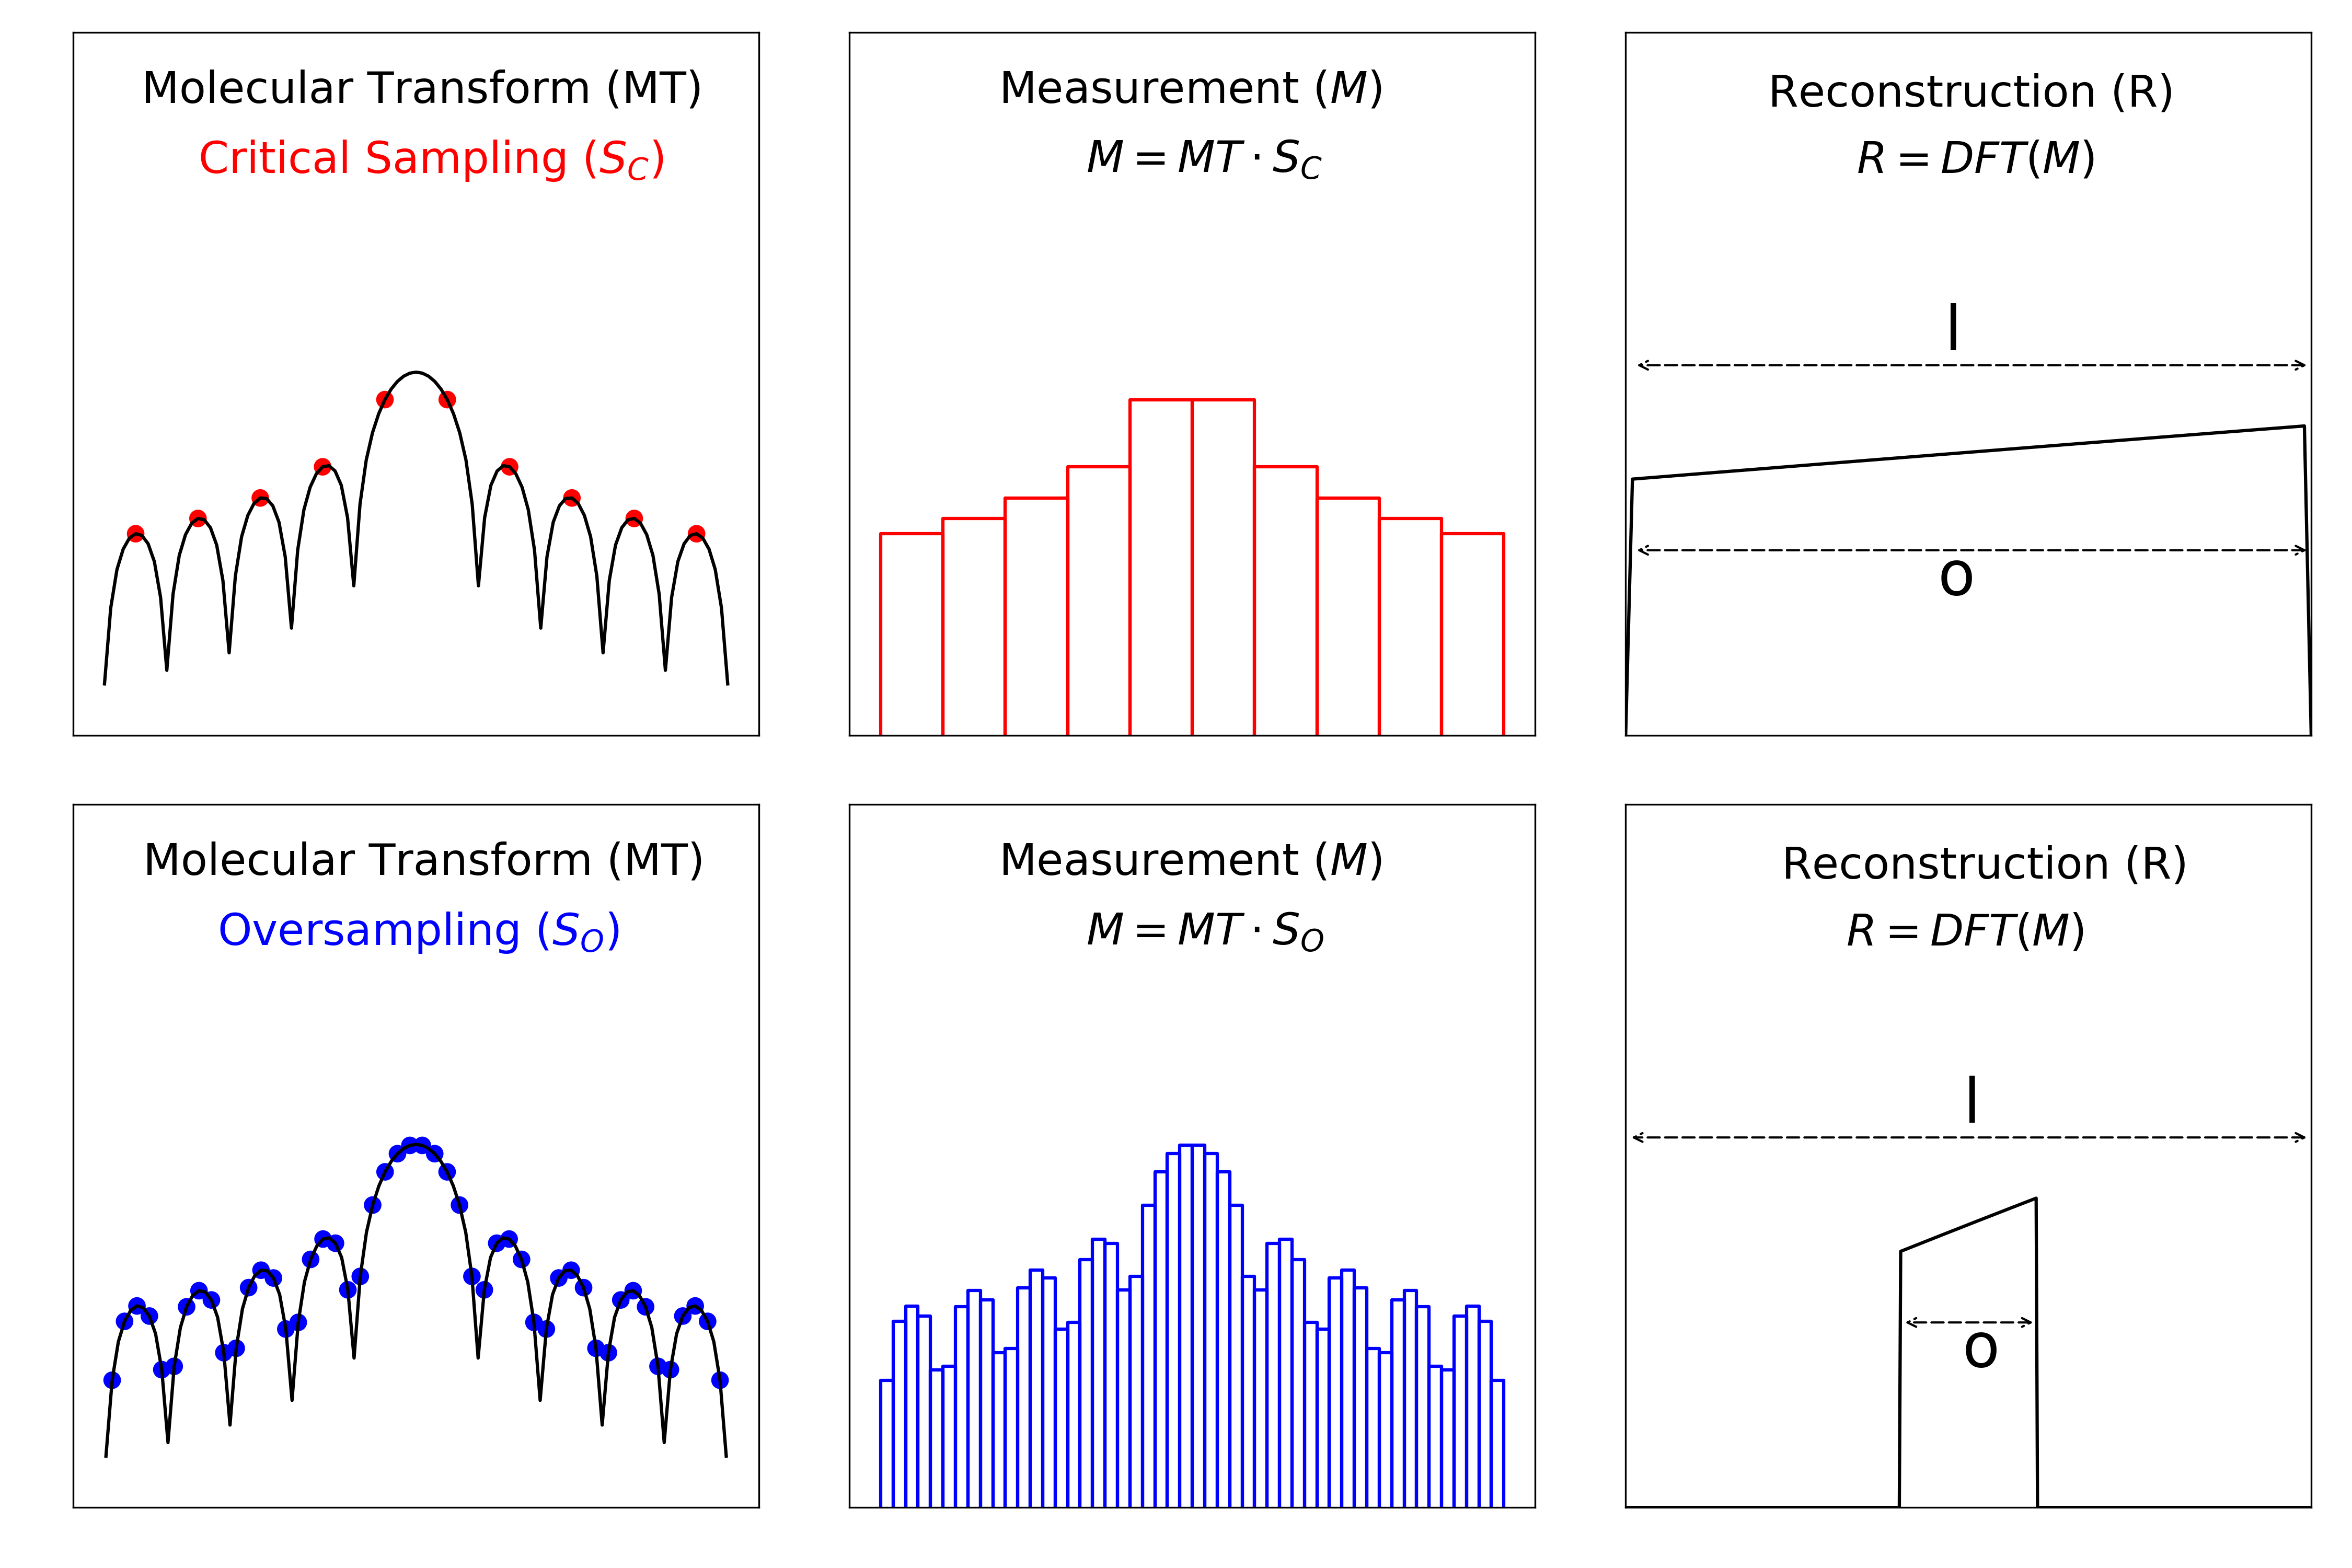
\includegraphics[width=120mm]{Chapter_06_Sampling.png}
	\caption{Illustration of critical sampling (top row) versus oversampling (bottom row).}
	\label{fig:sampling}
\end{figure}

The linear sampling rate $S$ is defined as the ratio of $l/o$, where $l$ is the window size, and $o$ is the object size. Due to the inverse relation between the object and the molecular transform $l = \frac{1}{q} = \frac{\lambda\, d}{p}$, where $q$ is a pixel in the molecular transform (see equation \ref{eq:q}). 

\begin{equation}
S = \frac{\lambda\,d}{o\,p}
\end{equation}

By choosing a detector setup such that the sampling rate is at least twice the critical sampling rate we can, in some cases, use the additional intensity information to recover the phases, and thus reconstruct the object from the measured intensities alone. It is known that this method does often does have multiple solutions in 1D \cite{Walther1963}, however, for higher dimensions it has been proven that, in most cases, an oversampled pattern will have a unique solution\cite{Bruck1979}. Oversampling is the basis of many phase retrieval techniques in SPI, as well as some clever phasing techniques in SFX \cite{Ayyer2016,Chapman2011}.

\section{Iterative Phase retrieval}
In practice there are many ways of possibly retrieving the phase information from the diffraction pattern, but most common phase retrieval techniques are variations of convex optimization algorithms. This section introduces the general idea behind convex optimization, and explains the working three different algorithms. It has to be appreciated that solving the phases problem in remarkably difficult. It is neither linear nor convex.

As with any difficult problem, one starts from the things that are known. Figure \ref{fig:sampling} shows that oversampling in Fourier space implies that there is an area the size of ($l-o$) around the object for which we know the electron density $\rho(\vec{r})$ is zero. This knowledge can be used as a constraint on the possible phases: we know that a correct choice of phases would make the corresponding $\rho(r)$ be zero in this area. The area that can contain positive electron density is called the support mask $M(\vec{r})$. This constraint is called the real-space constraint. Furthermore, we know that the recovered Fourier amplitudes should agree with the measured intensities. This is called the Fourier-space constraint. 

In 1978 Fienup \cite{Fienup1978}, inspired by an earlier algorithm by Gerchberg and Saxton [Gerchberg1972], introduced an algorithm called Error Reduction (ER) to solve the phase problem. ER is an iterative approach that tries to find the solution that minimizes the disagreement to both the real-space constraint and the Fourier constraint. In words it can be described as follows:\\
\begin{enumerate}
\item Assign random phases to each pixel.
\item Inverse Fourier transform F(s).
\item Set all electron density outside of $M$ to zero, keep other electron density.
\item Fourier transform $\rho(r)$
\item Make sure that the recovered amplitudes match the measured intensities. Keep the phases.
\item Go back to step 2.\\
\end{enumerate}


ER is sometimes able to find the correct solution, but because the problem is not convex, in general it often gets stuck in local minima, making ER unable to find the global solution.

In 1984 Levi and Stark realized that applying the above described constraints can be interpreted as projections in a multidimensional Hilbert space \cite{Stark1984}. Step 3 will from now on will be called the real-space projection $P_r$. A combination of step 4,5 and 2 will be called the Fourier Projection $P_f$.  In ER $P_r$ and $P_f$ can be defined as follows:
\begin{align}\label{eq:ER}
P_r \rho\left(\vec{r}\right) =& \begin{cases} \rho\left(\vec{r}\right) \quad &\mathrm{if}\,\,
    \vec{r} \in M\\0 \quad & \mathrm{if}\,\, \vec{r} \not\in M \end{cases}\\
P_f \rho(\vec{r}) =& \mathcal{F}^{-1}\left( \frac{\sqrt{I}}{|\mathcal{F}(\rho(\vec{r}))|}\mathcal{F}(\rho(\vec{r})) \right)
\end{align}

The largest difference between both projections is that the support constraint is convex, while the Fourier constraint is not. An iteration in ER can now been seen as a real-space projection followed by a Fourier projection. This can be summarized as:
\begin{equation}
\rho_{n+1}\left(\vec{r}\right) = \begin{cases} P_f\rho_{n}\left(\vec{r}\right) \quad &\mathrm{if}\,\,
    \vec{r} \in M\\0 \quad & \mathrm{if}\,\, \vec{r} \not\in M \end{cases}
\end{equation}

Two error metrics can be associated with both projection;the fourier error ($E_f$) and the real space error ($E_r$). $E_r$ is the fraction of density outside the support. $E_f$ shows the difference between the recovered amplitudes and the square root of the intensities. Mathematically $E_f$ and $E_r$ are defined as:

\begin{equation}
E_r = \left|P_r\rho(\vec{r}) - \rho(\vec{r})\right| = \left(\sum_i\rho_i^2\right)^{\frac{1}{2}}
\end{equation}

\begin{equation}
E_f = \left|P_f\rho(\vec{r}) - \rho(\vec{r})\right| = \left(\sum_{i}\left(\frac{\sqrt{I_i}}{|F(S_i)|}- F(S_i)\right)\right)^{\frac{1}{2}}
\end{equation}
  
\subsection{The Hybrid Input Output algorithm (HIO)}
In 1982 Fienup introduced an algorithm that can escape from local minima, the so-called the Hybrid Input Output algorithm (HIO). To achieve this HIO makes use of a so called relaxation parameter $\beta$. An iteration in HIO can be described as follows:
\begin{align}
\rho_{n+1}\left(\vec{r}\right) = \begin{cases} P_f \rho_{n}\left(\vec{r}\right) \quad &\mathrm{if}\,\,
    \vec{r} \in M\\\rho_n(\vec{r}) -\beta P_f \rho_n(\vec{r}) \quad & \mathrm{if}\,\, \vec{r} \not\in M \end{cases}
\end{align}

I see the $\beta$ parameter similar to temperature in simulated annealing. If $\beta$ is large even deep local minima can be escaped. Unfortunately this also means the global minima might be missed as well. If beta is small HIO will miss fewer minima, but will have greater difficulty escaping from them. As long as a minimum is not perfect ($E_r$ and $E_f$ are not both zero), HIO will, however, eventually be able to escape \cite{Martin2010}.

\subsection{The Relaxed Averaged Alternating Reflection algorithm (RAAR)}
Another algorithm that is used often in the work described in this thesis is the Relaxed Averaged Alternating Reflection algorithm (RAAR). RAAR does not escape all minima but it can escape shallower once. For high-quality data RAAR seems to find the solution quicker than HIO, and also in a more behaved manner. An iteration of RAAR can be described as follows:
\begin{align}
\rho_{n+1}\left(\vec{r}\right) = \begin{cases} P_f \rho_{n}\left(\vec{r}\right) \quad & \mathrm{if} \,\,
    \vec{r} \in M\,\mathrm{and}\,\rho_n(\vec{r}) \geq -(1+\beta)P_f\rho_n(\vec{r}) \\\
    \beta\,\rho_n(\vec{r}) -(1-2\beta) P_f \rho_n(\vec{r}) \quad & \mathrm{if}\,\, \mathrm{otherwise} \end{cases}
\end{align}

As both RAAR and HIO do not guarantee to end up in the bottom of a minimum, concluding phase recovery with a number of iteration of ER will ensure the bottom of the final minimum is found. This can improve the overall quality of the reconstruction, as shown in \textbf{Paper I}.

\subsection{Other algorithms}
There exist many other phase recovery algorithms. Examples are: diffusion map (DM) \cite{Elser}, GHIO[], HPR [], HAAR[] , ESPRESSO [], saddlepoint optimisation [], and charge flipping []. A software package called Hawk allows users to select and test different algorithms. Hawk is especially powerful as it is fast and directly gives graphical feedback about the reconstruction process. The latter can for example be very useful in determining the correct support size. 

\section{Shrinkwrap}
While HIO and RAAR perform well when the support is tight and well known, in practise this information is often not available. Phase retrieval can become impossible if the support is too large. In 2003 Marchesini developed an algorithm that does not require an \textit{a priori} known support as input, but instead tries to deduce the shape of the support during the reconstruction. It starts by guessing the support from the autocorrelation. It does so by blurring the autocorrelation and selecting all pixels above a certain threshold to be included in the support. Consecutively after each n iterations the support is updated by applying a Gaussian blur to the real space image and selecting the pixels that have a value above a certain threshold. By varying the amount of blur and/or the selection threshold as the iterations progress, the support can slowly wrap and shrink to the true shape of the object. The general idea behind the algorithm is that even with a non-accurate support some features will be recovered well, and by using these features finally the an accurate support will be found. The algorithm has been very successful for experimental data [].

\section{Validation}
In iterative phase retrieval every reconstruction results in an image, irrespective of it having biological relevance or not. It is therefore very important to have tools to validate a reconstruction. This section will describe different validation tools used in the field.

\subsection{Errors}
The most basic method to assess the difference in quality between two reconstructions is comparing the respective errors. The reconstruction with lower errors is generally considered to be a more successful reconstruction. This method however does not tell anything about the biological validity of a reconstruction and is most often only used to exclude outliers (reconstructions that have clearly failed).
 
\subsection{PRTF}
The standard tool to assess the quality of a reconstruction is the phase retrieval transfer function (PRTF). This function considers the variation within a set of independent reconstructions (each reconstruction starting from a random set of phases), and uses this variation to quantify the resolution of a reconstruction. The basic assumption behind the method is that if a similar object is retrieved repeatedly, this object is supposed to be similar to the true object. The variation between reconstructions is calculated for each pixel $i$ by adding all recovered amplitudes for that pixel and dividing the total vector by square root of the measured intensity for that pixel $v_i = |\frac{\sum A_i}{\sqrt{I_i}}|$. If the value of $v_i$ is close to unity all reconstructions recovered a similar amplitude for pixel i. The closer $v_i$ is to zero the more difference there is between individual reconstructions. The standard PRTF plot shows the radial average of $v_i$. A common practice is the field is to define the resolution of a reconstruction as the first time the 1D PRTF drops below $\frac{1}{e}$. This threshold is arbitrary. For spherical objects a periodic drop in the 1D PRTF, corresponding to a drop in measured intensity, can be observed. This drop can be explained by the fact that the phase of a pixel measuring 0 intensity is unconstrained.
 
\subsection{Missing Mode Analysis}
As described in previous sections diffraction patterns lack data. Even in the best case the central region will be missing because the direct beam will otherwise damage the detector. The main other sources of missing data are detector geometry and saturation. 

Reconstruction algorithms deal with this missing data by recovering the phase as well as the amplitude for the pixels in these regions. In many cases the missing data does not affect the stability of phase recovery, however this cannot be said in general. For this we have to note that the Fourier constraint does not limit the amplitudes in the missing data area, and the real-space constraint does not limit the electron density inside the support. If there exists an object that can fit inside the support and has a Fourier transform that is zero outside the missing data region, this object could be arbitrarily added to the solution and thus would form an ambiguity in the reconstruction process.

In general completely unconstrained objects do not exist. Objects that fit the support constraint and only slightly contribute outside the missing data region, i.e. weakly constrained objects, can however exist. In the design of an experiment, or when deciding whether or not to phase an object it is important to have a tool that predicts whether weakly constrained objects exist or not. Missing mode analysis is such a tool.

The DFT can be represented in matrix form, where each column represents a pixel in real space and each row represents a pixel in Fourier space. The rows and columns can be reordered according to whether they conform to the fourier and real space constraints or not.

\begin{equation}\label{equ:F_split}
  \mathcal{F} = 
  \left(\begin{array}{l|lll}
    \mathcal{F}_{SM} & &\mathcal{F}_{\bar{S}M}& \\\hline
    &&&\\
    \mathcal{F}_{S\bar{M}} & & \mathcal{F}_{\bar{S}\bar{M}} &\\
    &&&
  \end{array}\right)
\end{equation}

We are after objects that minimize $|\mathcal{F}_{S\bar{M}}\rho|$. A common method to find such objects is singular value decomposition [Eckart]. This method decomposes $|\mathcal{F}_{S\bar{M}}\rho|$ into a diagonal matrix $\Sigma$, and two unitary matrices U and V.



EXPLAIN EIGENVALUES AND BASIS




\subsection{Hierarchical clustering}
As the reconstruction process might end up in different solutions, we typically use the Fourier and real-space error to select what particles to keep for the PRTF. To test whether the Fourier Error and Real space error are good measures to assess the variance between individual reconstructions, we can compare the errors against how similar the reconstructed images are pixel-to-pixel. This can be done using a so-called clustering analysis. 

In \textbf{Paper I} we used the  UPGMA (Unweighted Pair Group Method with Arithmetic Mean) hierarchical clustering method [Sokal, Michener] to determine the number of structurally different solutions present in the set of reconstructions. The workflow of this method is illustrated in figure \ref{fig:UPGMA}.

\begin{figure}[h]
	\centering 
		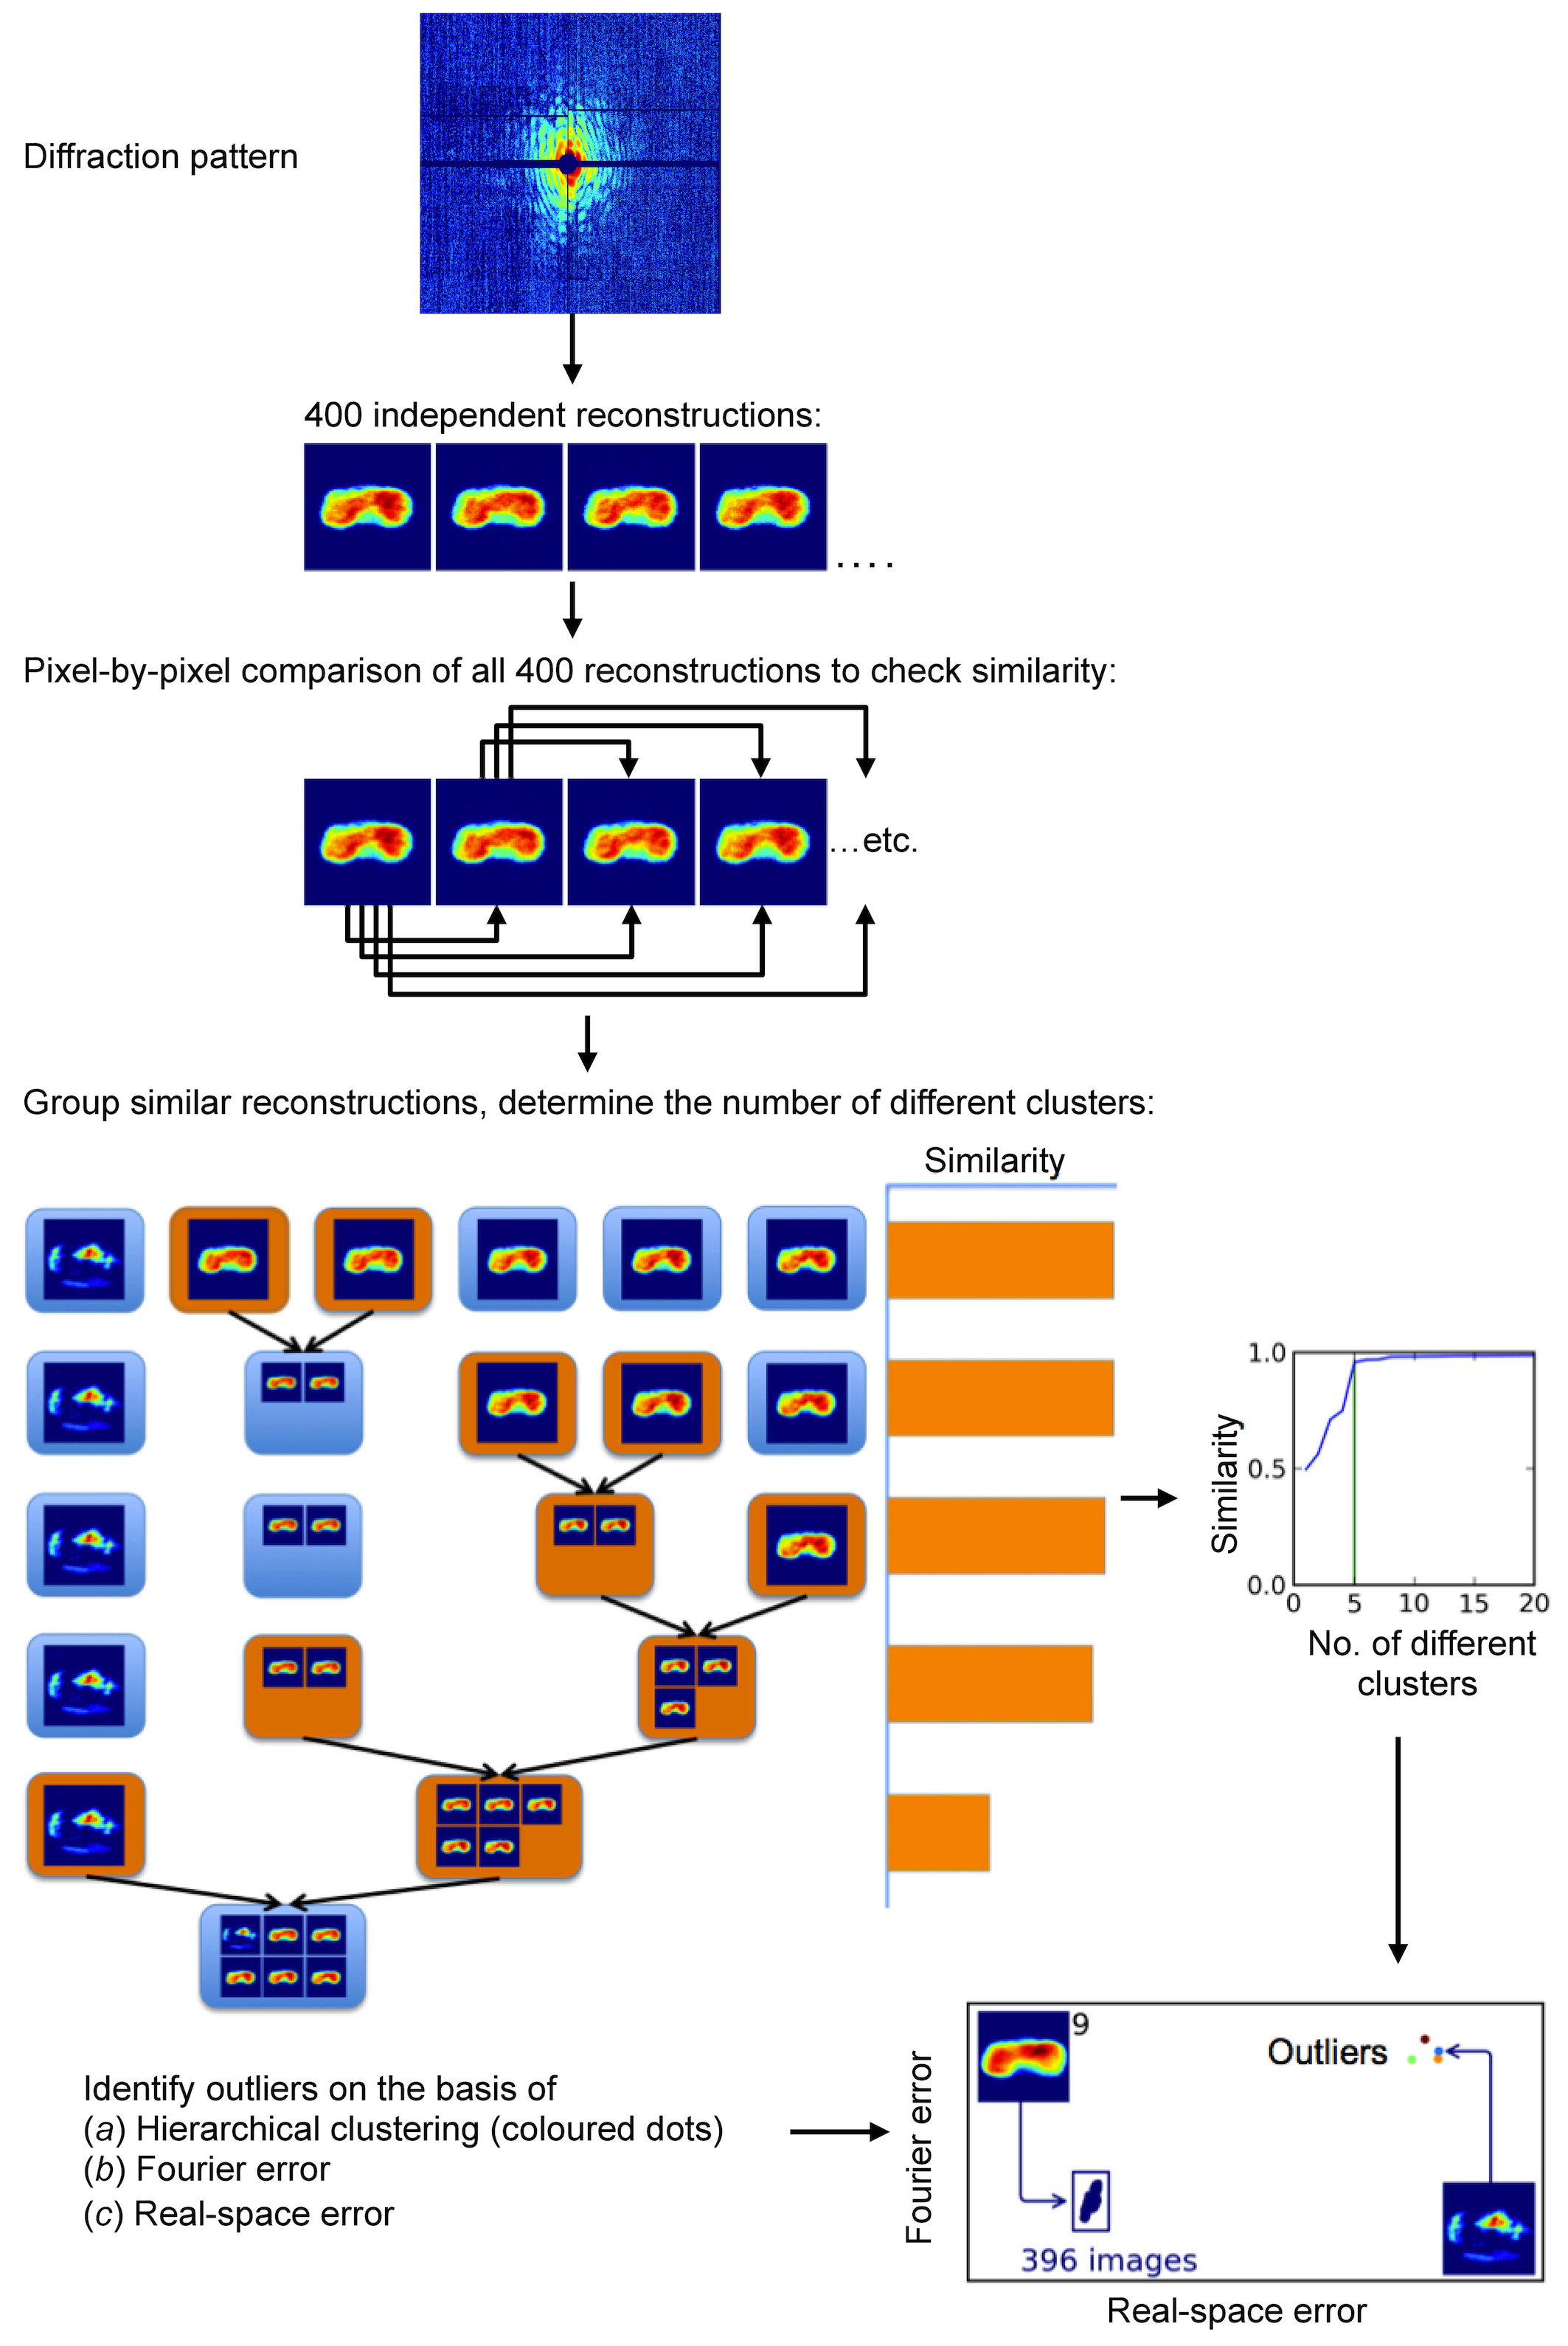
\includegraphics[width=100mm]{Chapter_06_UPGMAClustering.jpg}
	\caption{Flow chart of the UPGMA Clustering algorithm. In the first step of the algorithm, n independent reconstructions (400 in this example) are compared pairwise, pixel-to-pixel to check similarity. Each comparison results in a so called comparison score. The second step is the actual clustering step in which the number of different clusters present in the set of reconstruction is determined. Initially each reconstruction belongs to its own cluster. In each consecutive merging step the two most similar clusters are merged into one cluster. This repeats itself until one cluster remains. Each merge can be given a similarity score using the comparison	scores from step 1. By plotting the similarity scores against the number of clusters, the number of clusters can be determined. We choose the number of cluster by cheking where this plot makes a kink. This is indicated by the green line in the top graph on the right. The bottom plot shows the Fourier-error and the Real-space error associated to each reconstruction, color-coded on the basis of which cluster they belong to. Here we note that there are four outliers and one main cluster. The outliers are clearly failed reconstructions.}
	\label{fig:UPGMA}
\end{figure}

In the first step of this method each reconstruction is compared pairwise to every other reconstruction, pixel-to-pixel. The comparison score associated with each comparison is the normalized scalar product between the pair of reconstructions, after translating them to their optimal fit. 

In the second step of the method similar reconstructions are grouped in clusters. Initially each reconstruction belongs to its own cluster. In every consecutive step the two most similar clusters are merged into one cluster, until in the end only one big cluster remains. For each merge we calculate a similarity score, which is the average comparison score for all reconstruction in the merged cluster. We plot the similarity score of each cluster merge as a function of the number of clusters. The agglomeration step where the plot makes a "kink" is chosen as the number of different clusters that are present in the set of reconstructions. This is a standard way to estimate the number of clusters present in the set of reconstructions. This capability is an advantage of the  clustering algorithm. 

In a 2D plot of $E_f$ vs. $E_r$, color-coded by cluster, it is possible to see whether or not there is a correlation of reconstruction similarity and error score.  In the case that several large clusters remaining after applying a real-space error and Fourier-error threshold the clusters have to be examined carefully. If the remaining clusters correlate with the errors we suggest to keep only the cluster with the lowest error. If no correlation is present between score and cluster it is advised to keep all clusters for further evaluation. Otherwise there is a possibility of selecting on similarity, which would negate the validation power of the PRTF.

 
\section{Simulated Phase Contrast Methods}
Once one has retrieved the phase of the diffraction pattern, one has complete knowledge of the information encoded in the  wave-field. This total knowledge is powerful, because it allows the emulation of the action of any imaging system for which an associated mathematical transform can be written, regardless of its experimentally feasibility.
For example, differential interference contrast imaging, otherwise known as Nomarski imaging, is experimentally a well established technique to visualize the changes in phase. This change can have biological meaning, as for example the density inside certain organelles can be higher than the average density in cells. Normarski imaging will give a more pronounced image of the borders of the organelle. For an example see ref [mitochondrium). 

Nomarkski imaging in its simplest form takes a scattered wave-field, say $\psi(x,y,z = 0)$, and then interferes this wave-field with a copy of itself that has been given both a slight transverse displacement ($\Delta x$, $\Delta y$) and a phase shift $\phi_0$ (Nomarski and Weill,1955). Thus the intensity of the resulting wave-field $F_N$ is [Paganin]:
$|\psi(x,y,z=0)+ e^{(i\phi_0)} \psi(x - \Delta x,y - \Delta y,z=0) |^2$, from which one can show (using the Fourier shift theorem) that the transfer function becomes:
\begin{equation}
\begin{aligned}
\begin{split}
T_{DIC}(q_x, q_y, \tau) = 1 + e^{(i(\phi_0 - q_x \Delta x - q_y \Delta y))},\\
\tau = (\phi_0, \Delta x, \Delta y)
\end{split}
\end{aligned}
\end{equation}

In the case of a reconstructed image $\rho(\vec{r})$, the Normarski variant $N$ will look like:
\begin{equation}
N = \mathcal{F}^{-1} T_{DIC} \mathcal{F}(\rho(\vec{r}))
\end{equation}
We have created simulated Nomarski images of the reconstructed cell images shown in the results part.




    \chapter{Three dimensional Reconstructions}
So far we have dealt with two-dimensional diffraction patterns. Although much can be learned from two-dimensional images, a three-dimensional model is essential to understand the function of biomolecules.
From Chapter 2 we know that a diffraction pattern samples a curved slice through the center of the molecular transform of the object. If the same object would be illuminated from different angles, the resulting diffraction patterns together could sample the complete three-dimensional Fourier transform. The approach in which multiple two-dimensional images from different angles of illumination are combined into one three-dimensional image is called tomography.%This chapter will describe what possibilities there exist to recover the three-dimensional structure of bioparticles using single particle FXI. It will start by describing several methods that use o recover structure of particles that are reproducible in shape such as many viruses and rigid proteins, and after that discusses the poss

\section{Reproducible Particles}
In single particle FXI the illuminated particle is completely destroyed by the pulse. To date, it has therefore not been possible to image one particle multiple times using FXI. Some bioparticles however, are structurally reproducible. This means that diffraction patterns originating from different copies sample the same molecular transform, and can thus be combined to form the 3D fourier transform of the object. 

In order to successfully assemble the 3D molecular transform from multiple diffraction patterns, their relative orientations need to be known. Most of the time this information is unavailable as the sample delivery methods do not allow for orientation selection. A variety of reconstruction algorithms have been proposed for recovering the relative orientation of diffraction data, including the EMC algorithm \cite{Loh2009}, the manifold embedding (ME) set of algorithms \cite{Giannakis2010}, common-arc algorithm \cite{Bortel2011}, and multi-particle cross-correlation analysis \cite{Kam1977, Saldin2010, Kirian2011}. Theoretical studies suggest that the determination of diffraction pattern orientation should be possible even with photon counts as little as 100 scattered photons per image \cite{Loh2009}.

\section{The Common Arc algorithm}

Two diffraction patterns of the same object, will sample the same Fourier space. Because both diffraction patterns will slice the Fourier transform through the origin, both patterns must have at least an arc in common. The common arc algorithm uses this knowledge to find the relative orientation between two diffraction patterns. In short this algorithm can be described as follows. For each pair of patterns all possible arcs between the two pattern are compared and the best match is chosen as the true one. Based on the retrieved relative orientations between many pairs of patterns a full 3D model can be assembled. This method is successful as long as the diffraction patterns are not very noisy \cite{Tegze2012}. Too much noise makes the comparison between diffraction patterns unreliable.

\section{The expansion maximization compression (EMC) algorithm}
The expansion maximization compression (EMC) algorithm is an iterative algorithm. In each iteration the measured 2D diffraction patterns ($K_j$), where $j$ is the index of each pattern, are used to update a model of the molecular transform of the object ($M^{MT}$). The starting model can be chosen to be random, or if more is known about the model, this information could be incorporated. 

\subsection{Expand} 

Each iteration starts with the expand step in which the 3D model is expanded in all possible 2D slices throught the center, up to a specified angular accuracy. These slices are denoted $W_k$, where $k$ is the index of each slice. These slices represent the possible diffraction patterns given model $M^{MT}$. 

\subsection{Maximization} 

In the next step, each of the slices is compared to each diffraction pattern. This results in a matrix $R_{j,k}$ that describes how well each diffraction pattern fits in each orientation. The distance metric used for comparing the measured pattern to the predicted pattern often makes use of the noise type that affected the measurement. For instance, if you know that your measurement is only affected by shot noise one could use a Poissonian distance metric:
\begin{equation}
d_{Poisson}(W,K) = \frac{e^{-W_i}W_i^{K_i}}{K_i !}
\end{equation}
Here $i$ indicates the i-th pixel.

If you know your measurement is affected by a source that follows a Gaussian distribution $d_Gaussian$ can be used.
\begin{equation}
d_{Gaussian}(W,K) = e^{-\frac{(W_i-K_i)^2}{2\sigma^2}}
\end{equation}
Here $\sigma$ is the width of the noise distribution. Each slice in the expanded model is then updated by summing up the measured diffraction patterns weighted by the coefficients from $R_{i,j}$. This will localize the patterns to the orientations where they fit best.

\subsection{Compression}

In the final step a new model $M^{MT}$ is generated by putting back to updated slices $W_k$ in their respective orientations. This will enforce that the slices in the next expanded model will be internally consitent with each other.

\subsection{Fluence recovery}

So far we have assumed that the diffraction patterns from reproducible particles sample the same molecular transform. This is true as long as $E_0$, the strength of the x-ray pulse that hit the particle, is the same for each exposure. This we know is not the case (see Chapter 3). Due to the randomness of the SASE process the power of the pulse does fluctuate from shot to shot. Even if the total power of the pulse is known, it is unknown where in the pulse the particle was hit.Fortunately, EMC can also be used to recover this effective strength of the electric field using the following equation \cite{Loh2010}.
\begin{equation}
\Phi(K,W) = \frac{\sum_{j} R_{i,j} \sum_{i} K_{i,k}^2 }{\sum_{j} R_{i,j} \sum_{i} W_{i,j} K_{i,k}}
\end{equation}
This so-called scaling term $\Phi(W,K)$ is calculated each iteration after the maximization step. It is used in the maximization step to scale the diffraction pattern when construction a new model.

%Number of orientations

%According to [] the number of patterns that are required to assemble a model of the molecular transform at resolution $R$, which probability $p$ is:
%\begin{equation}
%N = \frac{ln(1-p^{1/K})}{ln(1-k/K)}
%\end{equation}


It is amazing how much noise EMC can tolerate, and still be able to retrieve orientations. This is true even if the noise model is not accurate. For the success of model assembly, it seems more important for EMC to, initially when the model is far from true, have the option to place diffraction patterns in a wide distributions of orientations, than it is to know the behaviour of the noise exactly.


%\subsection{Multi-model EMC}
%Often biomolecules are not static in their structure, but rather are flexible units, that structurally undergo small local changes, or sometimes even large global changes. So far FXI has not been shown to which means that the diffraction patterns sample the structural variation (or conformational landscape). This gives FXI the large potential of being able to map the conformational landscape of each protein, at room temperature. This makes it impossible to create one single structure from all diffraction pattern. Currently an EMC version is being developed that can be assemble multiple models from the data, and tries to deal with the structural heterogeneity is this way. It is very similar to single state EMC, but differs in the fact that it builds multiple self-consistent models. 
    \chapter{Image Classification}
In order for algorithms such as EMC to work, the amount of heterogeneity within the diffraction data set has to be limited. Furthermore, each of the steps in the experiment introduces its own type of noise to the measured diffraction pattern. For example think of the debris clumping around small particles compared to the drop when sprayed with the GDVN, detector malfunctioning or saturation, or intensity fluctuations due to the random start of the SASE process. Often the results of the first two types of noise can not be tolerated by EMC, and image classification before the EMC step is necessary. Also fast feedback about the first type of noise is very useful to have during the experiment. So far a very robust sizing method has been developed, but more extended methods might come in useful. Several methods shown here can give rapid feedback on the heterogeneity of the particle.

%\section{Template-based classification}
%If your object has a known shape it could be possible to only select the diffraction patterns that are similar to a set of expected diffraction patterns from the object called templates. Paper III explores the possibility of template-based classification. In general this method is highly dependent on the choice of template, as well as the amount and type of variation present in your sample.

\section{Feature extraction}
A way of selecting diffraction patterns is by extracting general features from the diffraction pattern such as size, particle shape, amount of saturation, number of particles in the beam. Based on the relative values associated with the features individual patterns might be selected or discarded, or if these values are determined during an experiment, the experimental conditions might be rapidly adjusted. This section describes several feature extraction algorithms I have implemented.

\subsection{Size}
A common method to determine the size of an object is fitting the central speckle to the central speckle of simulated diffraction pattern from a sphere. This method has shown to be successful for particles that have an icosahedral to spherical shape \cite{Hantke2014,Daurer2017}. If the 3rd to the 5th minima are also present in the diffraction pattern, the average of these minima can also be used to determine the size of the object. This method can be especially useful in case the central speckle or first minimum cannot be evaluated reliably due to for example saturation effects. Figure \ref{fig:sizing} shows the relative reliability of using different minima to assess the size of an icosahedral object. These results rely on simulated diffraction patterns \cite{Hantke2016}.

\begin{figure}[h]
\centering
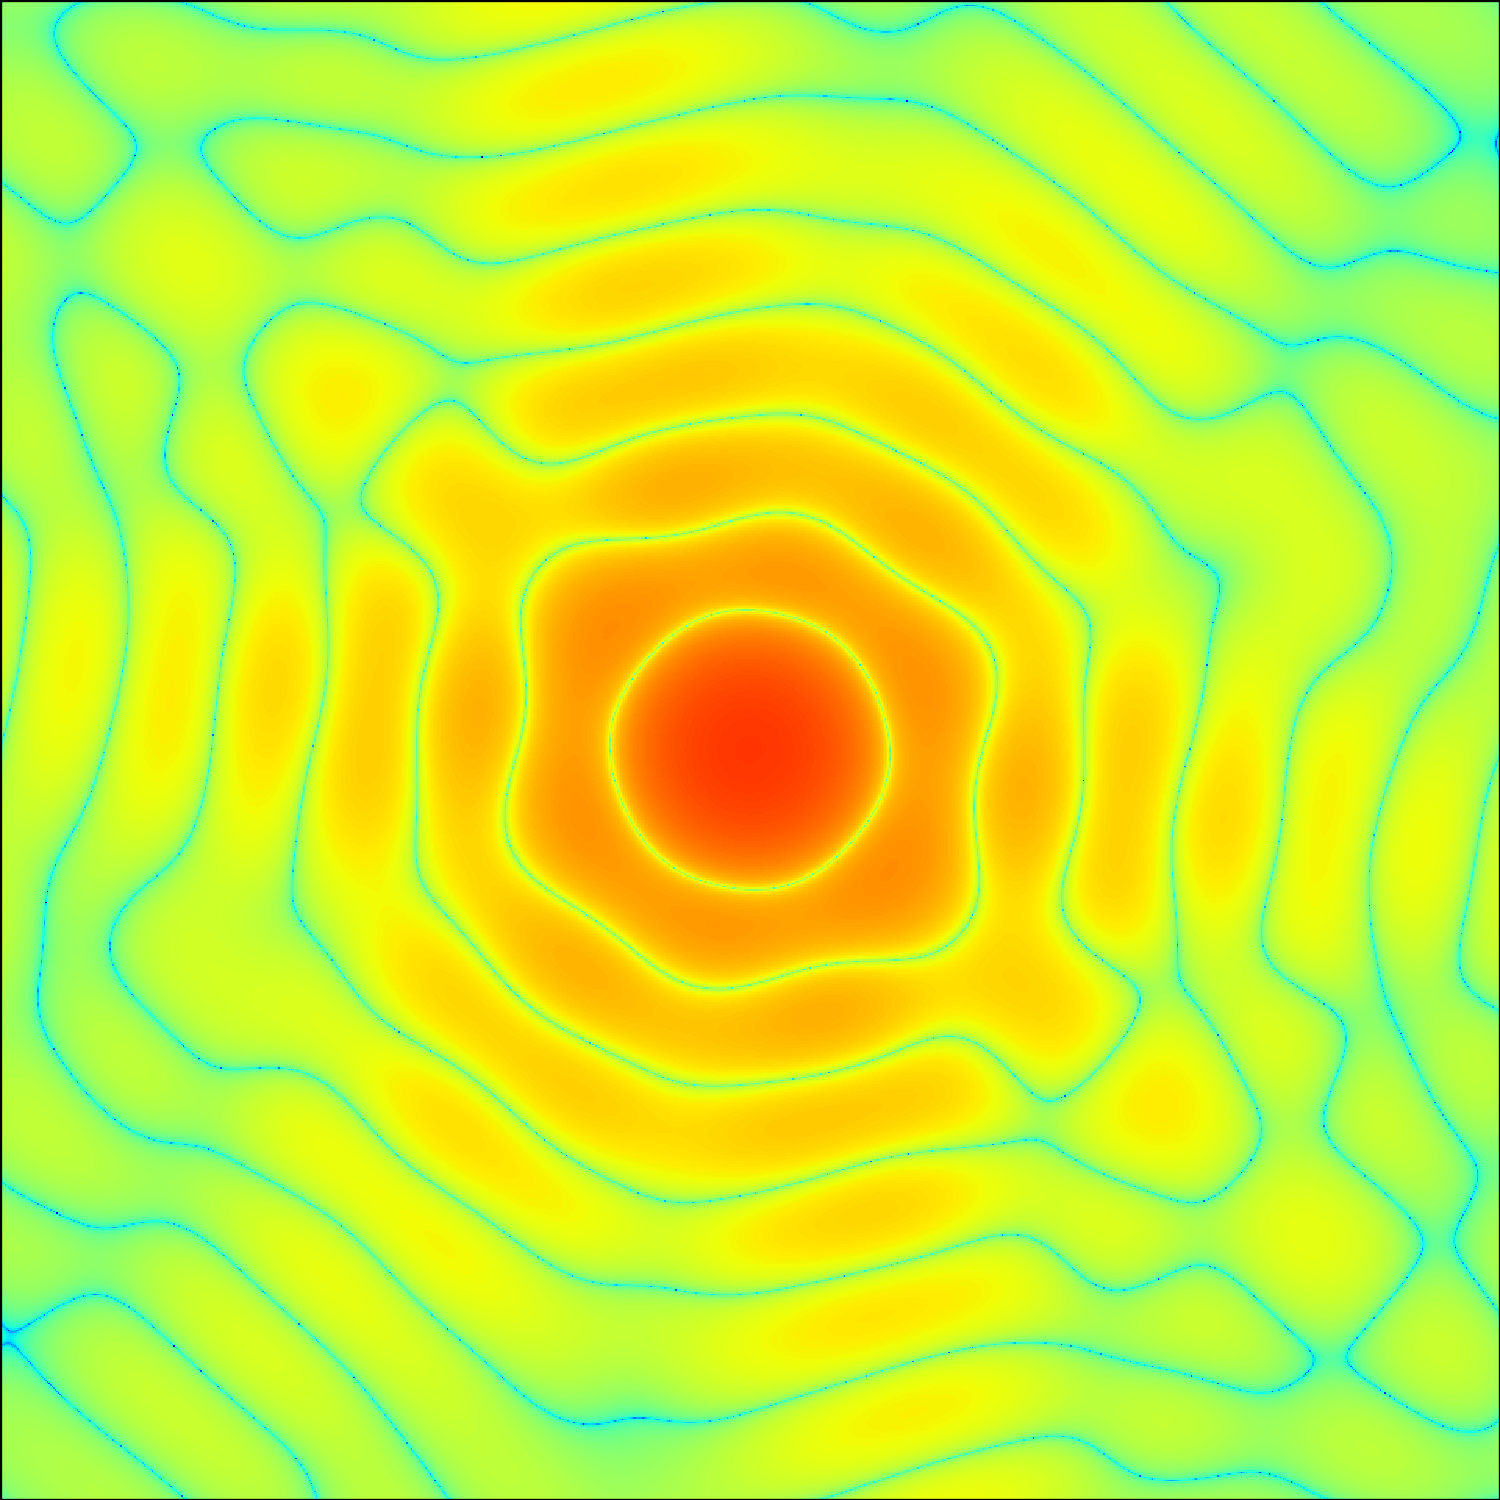
\includegraphics[width=42mm]{Chapter_08_ImageClassification_Simulated_Icosahedron.png}
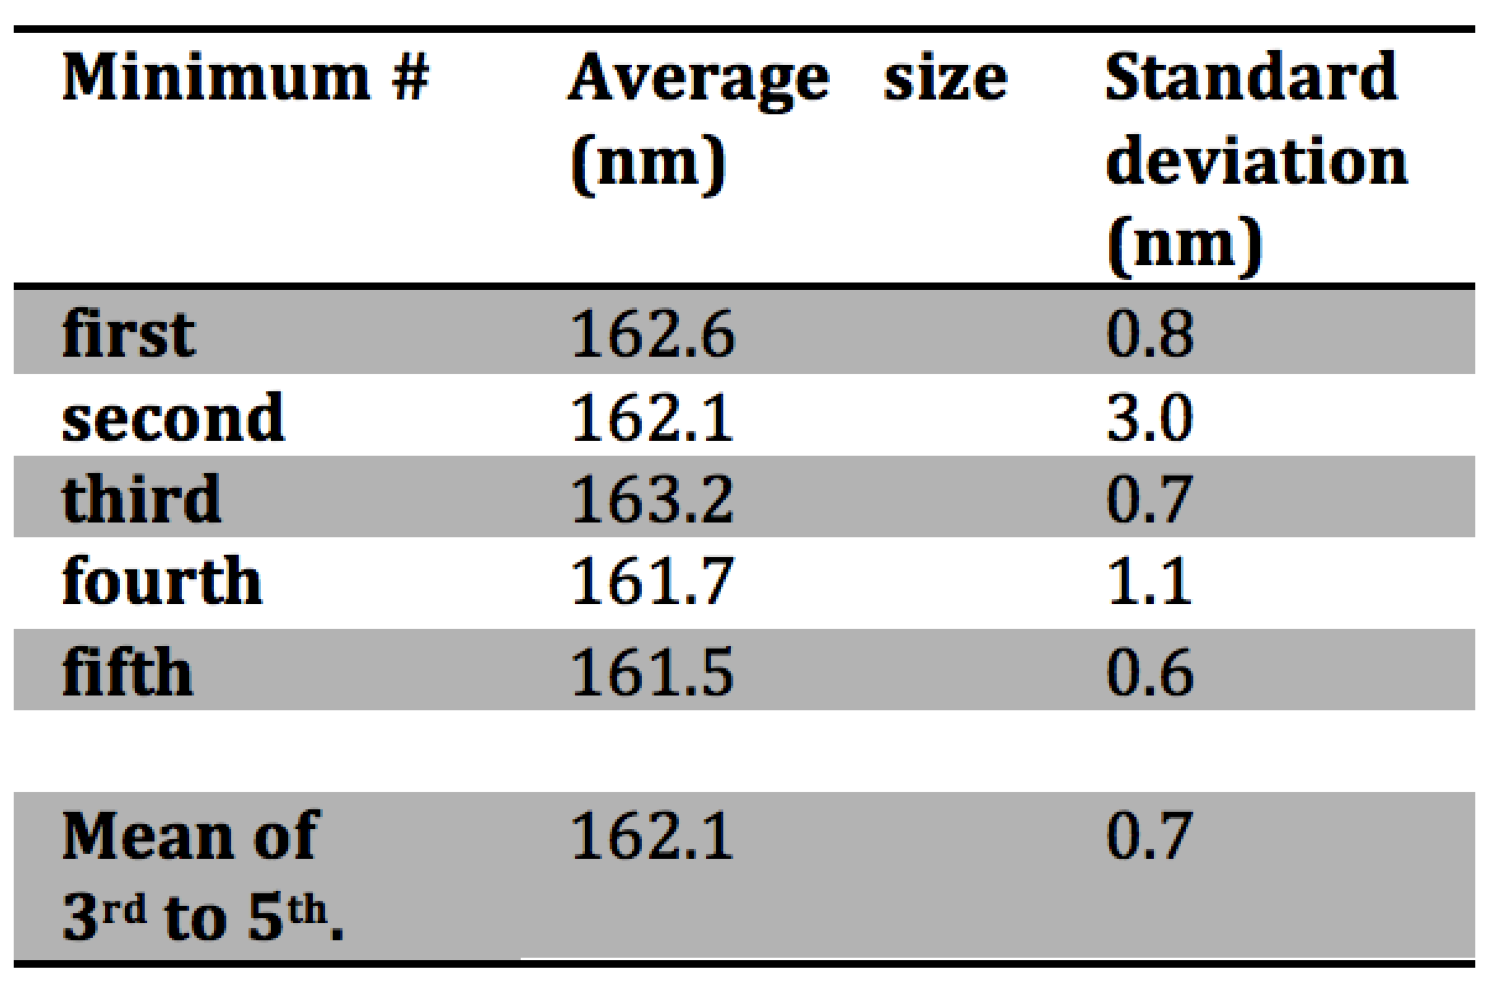
\includegraphics[width=65mm]{Chapter_08_ImageClassification_Stats.png}
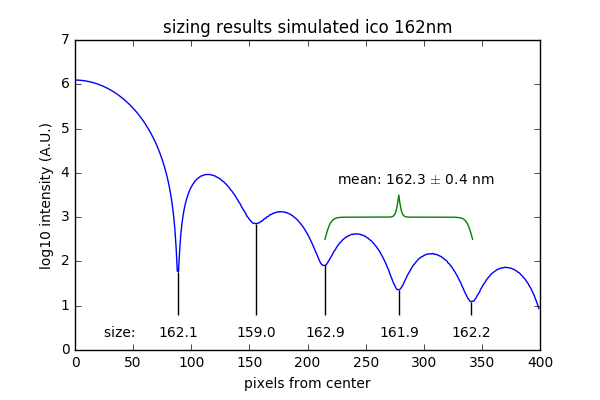
\includegraphics[width=100mm]{Chapter_08_ImageClassification_Sizing_Results.png}

\caption{Evaluation of the size assessment of a icosahedrally shaped particle of 162 nm, using the location of different minima. a) An example of the simulated diffraction patterns used in this evaluation. Each diffraction pattern has a random orientation with respect to the beam. b) The radial average of the diffraction pattern a) with associated size estimates corresponding to the location of each minima. c) the average size estimates based on the location of the each minima, and their respective standard deviations. Although the first minimum is the best in determining the size of an object by itself, the mean of the 3rd - 5th minima are also very good in determining the size of the object.}\label{fig:shape_assessment}
\end{figure}


\subsection{Edge detection}
Some objects are characterized by having sharp edges. A sharp edge in real space corresponds to a streak in the direction perpendicular to the edge in Fourier space. Objects and/or orientations of objects might be classified by determining if streaks are present, and how many. Figure explains the idea behind a streak finding algorithm.

\begin{figure}[h]
\centering
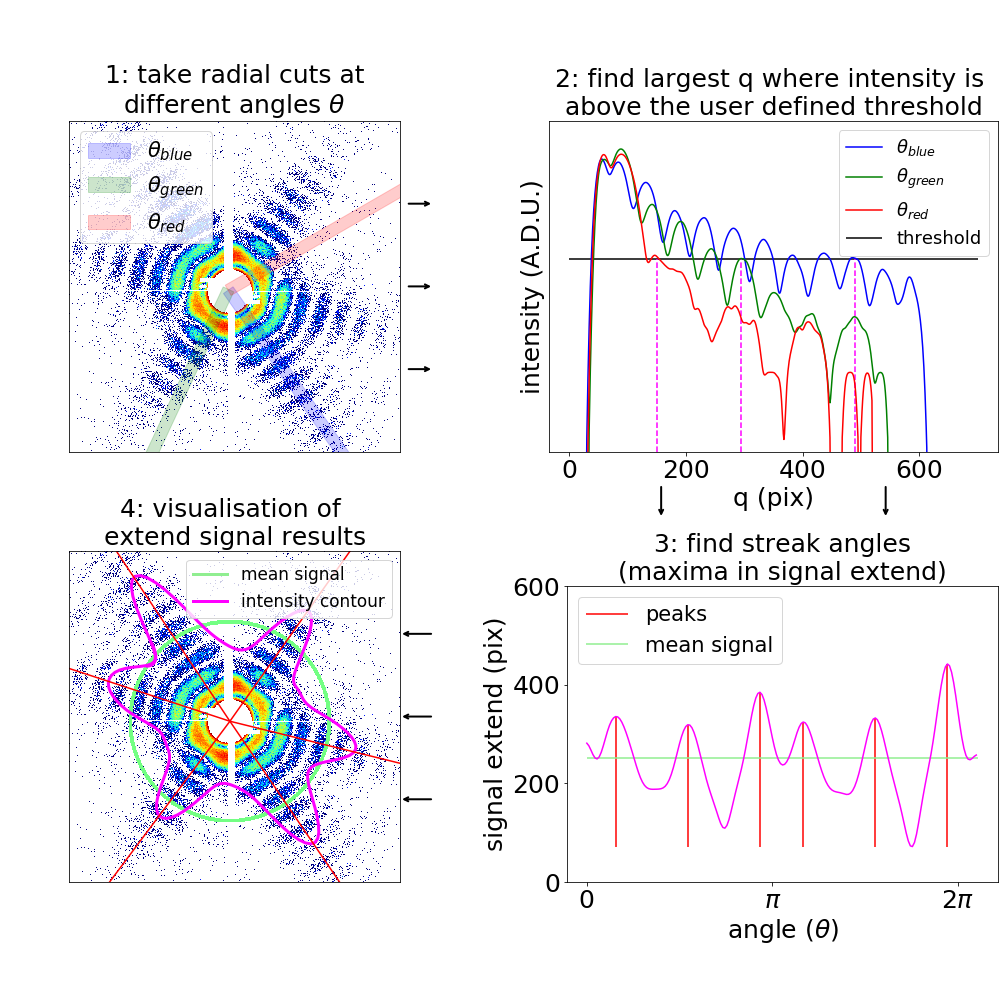
\includegraphics[width=120mm]{Chapter_08_ImageClassification_Edge_Detection.png}
\caption{An evaluation of where in the diffraction pattern the signal is located. In the first step radial cuts are taken each \textit{n} degrees. In 1) only three cuts are visualized: the blue cut is on a streak, the green one is on the edge of a streak, and the red one is in between two streaks. In step 2 the largest distance from the center where the intensity is above a user-defined thereshold is determined. These points are indicated by the dashed magenta lines in 2). The three cuts from 1) show a difference in signal extend. In step three the maxima in the signal extend are determined (see 3). If a maximum has a 180 degree pair, we consider the pair coming from a streak. The average signal extend is indicated by the lightgreen line. 4) The magenta lines contours the signal extend in the diffraction pattern. The red lines indicates the streak location and the lightgreen circle is the mean signal level.}\label{fig:edge_detection}
\end{figure}

\subsection{Elongation}

It might also be possible to determine the elongation of the particle, either by evaluating the elongation of the central speckle \cite{Hantke2014,Daurer2017} or by evaluating the elongation of the central term in a filtered autocorrelation. This is useful in discerning between diffraction from spherical and non-spherical objects. Figure \ref{fig:shape_assessment} shows two diffraction patterns: A and B. Diffraction pattern A originates from a icosahedral object and thus has a round central speckle (CS\_A). The fraction of the shortest distance from the center of the central speckle to the edge of the central speckle (minor) divided by the longest distance is called the elongation $\epsilon_{DP}$. Round central speckles have an elongation of 1. The central speckle of pattern B (CS\_B) is much more elongated. 

The evaluation of both the autocorrelations show a similar trend. AC\_A shows a roundish particle, whereas AC\_B shows a density that is more elongated. In the radial average of AC\_A and AC\_B this becomes visible as a mass beyond the maximum. The green area is considered to be part of a round particle, and the red area is considered to be part of an elongated particle. The fraction of the green area divided by the green plus the red area constitutes the elongated parameter $\epsilon_{AC}$ \footnote{Of course both these methods does not say anything about the elongation of the particle in the direction of the beam.
} The autocorrelation can only be used for the evaluation of convex objects, as non-convex object might appear roundish. 

\begin{figure}[h]
\centering
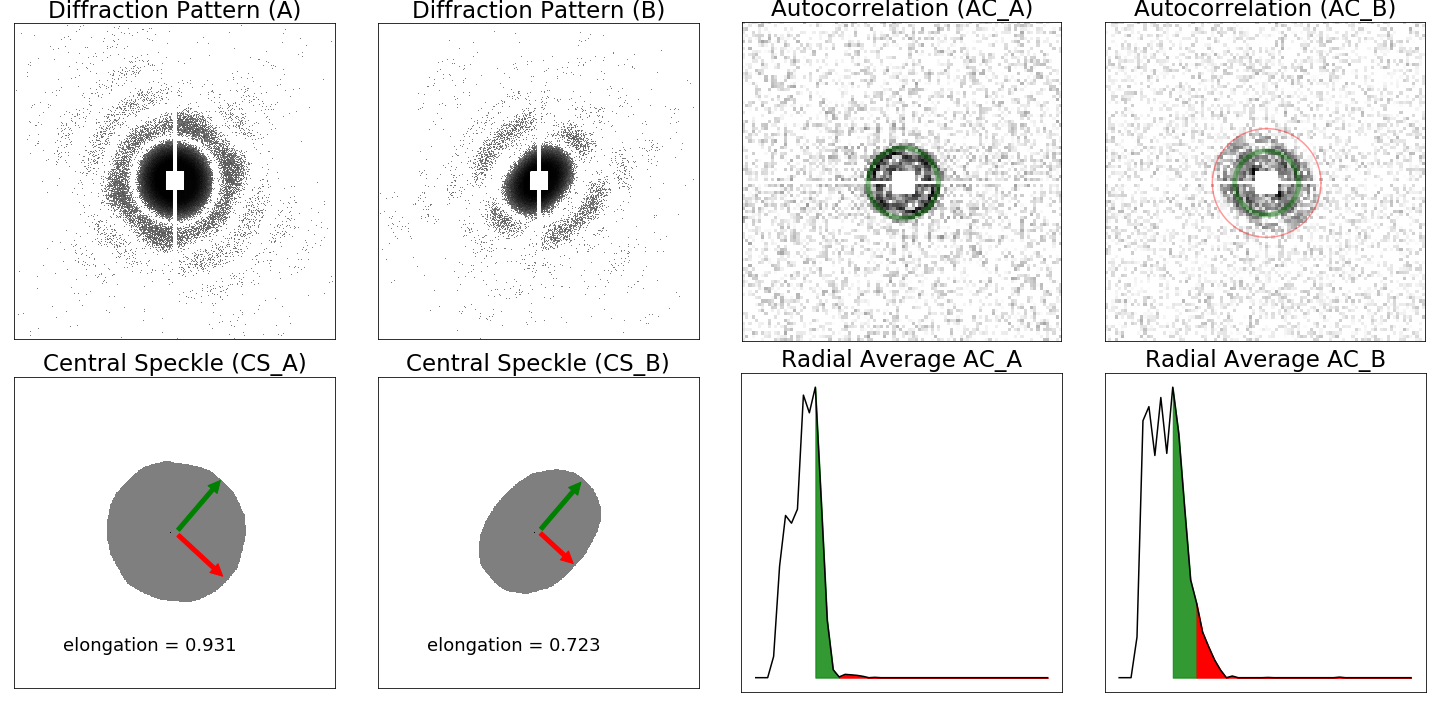
\includegraphics[width=120mm]{Chapter_08_ImageClassification_shape_assessment.png}
\caption{Elongation assessment of the particles that gave rise diffraction pattern A and B. From the central speckles of A and B, CS\_A and CS\_B, have a different shape. The elongation factor $\epsilon_{DP}$ is the fraction of the minor over the major axis of the central speckle. If $\epsilon_{DP}$ is close to 1, the objects that gace rise to the diffraction pattern is considered round in projection. The smaller $\epsilon_{DP}$ the more elongated the particle is considered. The evaluation of the autocorrelation plots show similar results. The central blob in AC\_A is roundish, whereas the central blob is more elongated in AC\_B. In the radial averages of both AC\_A and AC\_B the size of the object is taken as the maximum. The green density is considered part of a spherical object. The red density is considered part of an elongated object. $\epsilon_{AC}$ is the fraction between the green area over the green area + the red area. The closer this fraction is to 1, the more round the particle is considered.}\label{fig:shape_assessment}
\end{figure}


\subsection{The shape of the particle}
Particle shape or at least the particle size is important for automated phasing. So far automated routines have mainly dealt with icosahedral or round particles, as the size determined from the central speckle is enough to determine an accurate support constraint \cite{Hantke2014,Daurer2017}. The support size (and shape) of elongated particles such as most cells and many virus species cannot be accurately guessed in this way. This section introduces a method that can make a rough support guess for elongated particle by tracing the contour of the central term of in a filtered autocorrelation. This method uses a Lorentz based edge detection \cite{mathworks2018}.
Figure \ref{fig:detailed_shape_assessment} shows an example of how particle shape assessment using Laplace edge detection performs.

\begin{figure}[h]
\centering
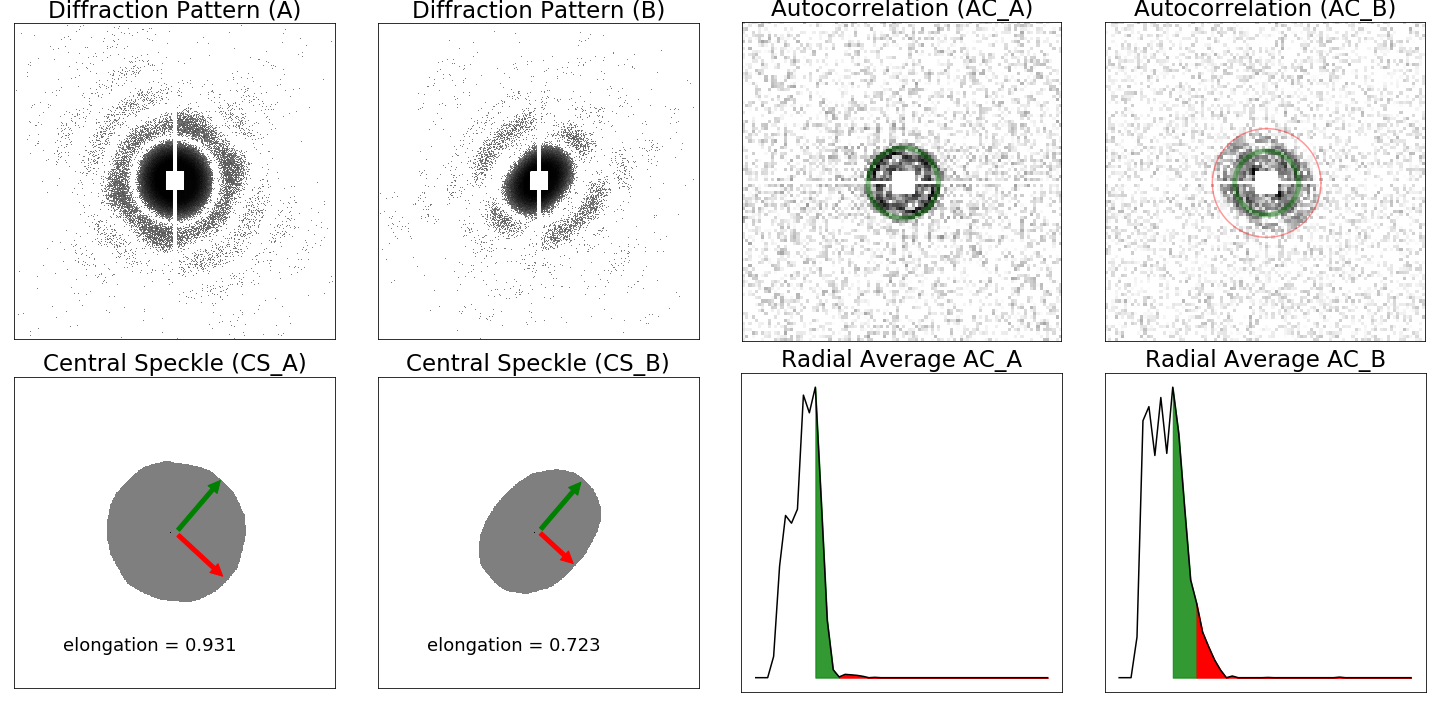
\includegraphics[width=120mm]{Chapter_08_ImageClassification_shape_assessment.png}
\caption{Finding the shape of the particle. a) shows the filtered autocorrelation of the particle. b) shows the autocorrelation after applying the laplacean edge detection. c) shows the selected area within the autocorrelation. It matches the central term of the autocorrelation. This shape can be used to determining the major and minor size of the particle, and possibly as a guess for the support or support size. }\label{fig:detailed_shape_assessment}
\end{figure}


\subsection{Multiple scatterers in the focus}

Due to the stochastic nature of the injection method, two particles can end up in the interaction region at the same time. If the particles are attached to each other, a similar pattern as seen in figure \ref{fig:shape_assessment} will occur. If the two particles are separated in space, the scattered signal of the two particles will interfere. As a result so called Newton rings will be observed in the diffraction pattern (See Figure \ref{fig:moire_pattern}. These rings code for phase information, that simply can be retrieved from the autocorrelation, as shown in Paper XX. The resolution of the reconstruction will be related to the size scatterer, the amount of missing data, and the strength of the signal. Without going into detail as to why this is the case, it can be easily understood that such patterns should be separated from the patterns originating from single particles. This section describes a method that identifies patterns coming from multiple scatterers, by identifying the presence of non central terms in the autocorrelation (these are so-called holograms). 

The first method will calculate the autocorrelation plot of the diffraction pattern, mask areas that are heavily affected by artefacts, and subtract the autocorrelation of a representative diffraction pattern. The latter is done to limit the main source of noise in the autocorrelation plot, originating from the missing data. Based on the size estimate of the particle, a central area is also masked. The error score associated with whether there are two particles present simultaneously in the focus is called $\Sigma_{HF}$. $\Sigma_{HF}$ is the median value in the autocorrelation divided by the maximum. If $\Sigma_{HF}$ is close to 1, there is most like only one particle in the beam. A threshold of 0.9 is regularly taken as the threshold for the presence of multiple particles, separated at a distance from each other.

As method one is limited in observing holograms that are located closely to the central term, a second method is needed. In this method the autocorrelation is calculated for small patches of the diffraction pattern (See Paper XIX). The advantage of selecting  patches is that their location can be chosen such that these autocorrelation plots will be less affected by possible missing data. The error metric $Sigma_{HP}$ is calculated in the same way as $\Sigma_{HF}$. The threshold for $\Sigma_{HP}$ is usually 0.3. It may however be the case that the interference structure is rather faint, such that none of the selected patches detect it. In this cases the former method for multiple selection has a higher chance to succeed.

Figure \ref{fig:Multiple_distance_assessment} shows an example of how particles are evaluated using the two methods. The left most panel shows the measured diffraction pattern. Notice the circular rings that have a center somewhere beyond the top right corner. These rings are the interference terms of the two particles. b) shows the autocorrelation of the full pattern a, after subtracting the autocorrelation of the diffraction pattern of an average particle (reference particle), and masking a central region, and a central cross. The latter also reduces artefacts. c) shows the autocorrelation of a small part of the diffraction pattern. This autocorrelation is generally less tainted by artefacts, but for weak interference signal a small region might be too small to pick up a significant signal.

\begin{figure}[h]
\centering
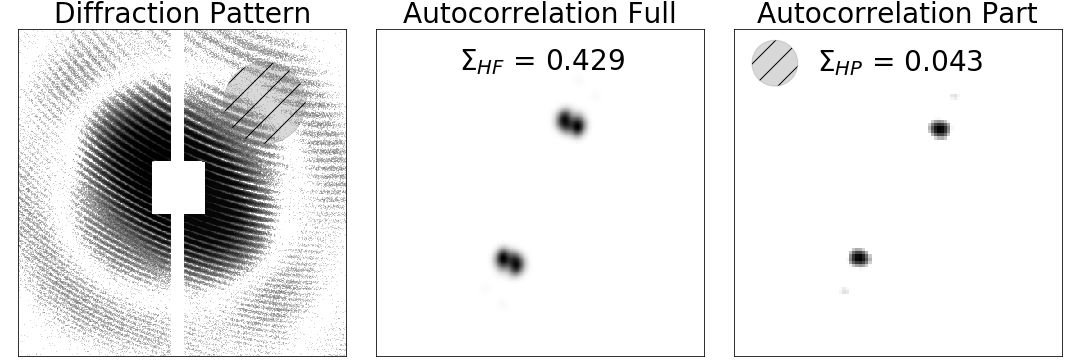
\includegraphics[width=120mm]{Chapter_08_ImageClassification_Multiple_Finding.png}
\caption{Assessing the prescence of multiple particles in the focus, located at a distance from each otherFinding the shape of the particle. a) shows a diffraction pattern which has clear circular interference rings present (center of the rings are somewhere beyond the top left corner. Note the gray circular area. This area of the diffraction pattern is used in c). b) shows the autocorrelation of a) after subtraction an average autocorrelation. The subtraction helps to reduce artefacts coming from the missing data. c) shows the autocorrelation of a small circular area in a). Both methods give two peaks.  }\label{fig:detailed_shape_assessment}
\end{figure}
    \chapter{Experimental Results}
\section{Imaging live cells}
For the study described in \textbf{Paper I} we used cells of two species of cyanobacteria: \textit{Cyanobium gracile} and \textit{Synechococcus elongatus}. Cyanobacteria are photosynthetic bacteria that can be found in almost any habitat on earth, ranging from hot volcanic areas to cold polar ice caps, and play an important role in the global carbon and nitrogen cycle. In a 25 day cycle an algal bloom of 1000 $km^2$ can sequester around 22,000 tonnes of atmospheric carbon into organic carbon before an infection by cyanophages cause the bloom to collapse \cite{Lehahn2014}.
 
\textit{Cyanobium gracile} cells were selected for this experiment because of their small size and their robustness with respect to the injection procedure. Single \textit{C. gracile} and \textit{S. elongatus} cells have an oval-to-cylindrical shape, and vary in size between 0.25-0.4 $\mu$m in diameter and 0.4-4.0 $\mu$m in length \cite{Komarek1999}. Cells divide symmetrically by binary fission. The two daughter cells separate from each other after reaching the size and shape of the mother cell \cite{Bazire1988}. We used non-synchronised cell cultures undergoing active growth, which means our sample contained cells in various stages of their cell cycle. 

%\subsection{Data Collection}
The experiments described in \textbf{Paper I} were carried out at the atomic, molecular, and optical science (AMO) endstation at LCLS \cite{Bostedt2013}, at a photon energy of 512 eV (corresponding to a wavelength of 2.40 nm) and 1100 eV (1.13 nm). Figure \ref{fig:experimental_geometry} shows the arrangement of the experiment. The length of the photon bunch was about 70 fs. Far-field diffraction patterns were recorded on a pair of pnCCD detectors \cite{Struder2010} in the CFEL-ASG Multi Purpose (CAMP) instrument \cite{Struder2010}. The detectors were place at 741 mm downstream from the intersection between the X-ray beam and the stream of sample. The detector read-out rate matched the 120 Hz repetition rate of the LCLS. 

We collected diffraction patterns of \textit{C. gracile} cells for an hour at a hit ratio of 43\%. The strongest 7,500 hits were selected for further analysis, using the Cheetah software package \cite{Barty2014}. The linear sampling ratio of the particle was around 20-fold, which allowed direct phase recovery from the measured intensity patterns. Phase retrieval was not a trivial problem because strong hits saturated the detectors at low diffraction angles. As a compromise, we manually selected medium-strong hits, which contained either no, or only few saturated pixels, while still providing scattered signal to reasonably high resolution. Missing mode analysis revealed no unconstrained modes for all reconstructed cells presented in \textbf{Paper I}. 

Phases were retrieved using the Hawk software package \cite{Maia2010}. For each pattern 400 reconstructions were made, each starting from different random initial phases. These reconstructions consisted of 5000 iterations with the RAAR algorithm \cite{Luke2005}, using a Shrinkwrap algorithm \cite{Marchesini2003} for support determination, and concluded with 100 iterations with the ER algorithm \cite{Fienup1978, Fienup1982}. The initial and final support sizes were manually determined. No real-value constraints were used since we anticipated the effects of absorption in the thick cells to give effects similar to a phase object. 

\begin{figure}[!ht]
	\centering 
		\includegraphics[width=120mm]{FF.png}
	\caption{Diffraction patterns and reconstructed electron densities for live C. gracile cells. The cells were alive when the femtosecond pulse traversed them but exploded some picoseconds later. Photon energy: 517 eV (water window), sample-to-detector distance: 740 mm. The total number of scattered photons in the diffractions patterns varies between 0.5 and 5 million. Each reconstructed image is the average of up to 400 independent reconstructions. Resolution was estimated from the phase retrieval transfer function. White circles in the reconstructions indicate the resolution relative to the object size. Feature smaller than the circle should not be interpreted as sample features. Reconstructions are normalized, where dark blue is 0 density and dark red is the most dense part of the cell.The cells are sorted according to cell size. Synthetic X-ray Nomarski images were calculated from the complex-valued reconstructions to show the reconstructed phase shift properties of the object together with its density.}\label{fig:Reconstructions}
\end{figure}

Figure \ref{fig:Reconstructions} shows the reconstructed exit wave-fronts for six \textit{C. gracile} cells together with the corresponding diffraction patterns, and a synthetic Nomarski image. The reconstructions represent 2D projections of the electron density of the cells. The images show the expected morphologies of cells during division \cite{Komarek1999,Bazire1988}. The resolution of each reconstruction is indicated by the size of the round white dot. This means that features smaller than the dot were not recovery reproducibly and should not be interpreted as features of the sample.

\begin{figure}[!ht]
	\centering 
		\includegraphics[width=120mm]{prtf.png}
	\caption{Image resolution of the reconstruction. For each reconstruction shown in Fig. \ref{fig:Reconstructions}, the corresponding PRTF is shown. Resolution is determined as the first time the PRTF function drops below 1/e \cite{Seibert2011}. The white dot in the reconstruction has the size of the resolution determined from the PRTF.}
	\label{fig:PRTF}
\end{figure}

The resolution of the reconstructions were estimated from the PRTF (See Figure \ref{fig:PRTF}), using the 1/e threshold. Before calculating the PRTF and averaging the repeated reconstructions we removed outliers between the reconstructions by applying a threshold to the Fourier error. Clustering validates the results from using a threshold on the Fourier error and the real-space error. On average the main cluster contained about 370 out of 400 reconstructions (93\%), except for one case where only 96 reconstructions formed the biggest cluster (Figure \ref{fig:Clustering}). That the main cluster often incorporates most reconstructions, and has the lowest error scores made us believe that the average image of the main cluster is likely to represent the best reconstruction minimum. 

\begin{figure}[!ht]
	\centering 
		\includegraphics[width=120mm]{Clustering.png}
	\caption{Scatter plots of the Fourier vs real-space error for each individual reconstruction for each average reconstruction shown in Fig. \ref{fig:Reconstructions}. Each cluster has its own color. The image in the top left corner is the average reconstruction of all the reconstructions selected within the blue box. The threshold for cluster selection has always been the Fourier error, which avoids selecting for similarity. }
	\label{fig:Clustering}
\end{figure}

Detector saturation limited the achievable resolution. A number of much stronger exposures than shown in Figure \ref{fig:Reconstructions} were also recorded, and in some of these exposures the diffraction signal extended to nanometer resolution. Figure \ref{fig:StrongHit} shows one such pattern for a live \textit{S. elongatus} cell at 1,100 eV photon energy. Two pnCCD detector pairs were used to record this pattern. The configuration of the central back detector in Figure \ref{fig:StrongHit} is identical to the detector to record the diffraction patterns shown in Figure \ref{fig:Reconstructions}. The front detector is the same type as the back detector but is placed at 220 mm from the interaction region. In strong exposures, a large part of the back detector was saturated, which prevented reliable phasing. The signal however extended beyond 4 nm resolution on the front detectors, which is the size of a small protein molecule. More than 58 million scattered photons were recorded on the back detectors, and 1.3 million on the front detectors. The size of the cell was derived from the autocorrelation, shown in the boxed panel in the middle of Figure \ref{fig:StrongHit}. 

\begin{figure}[!ht]
	\centering 
		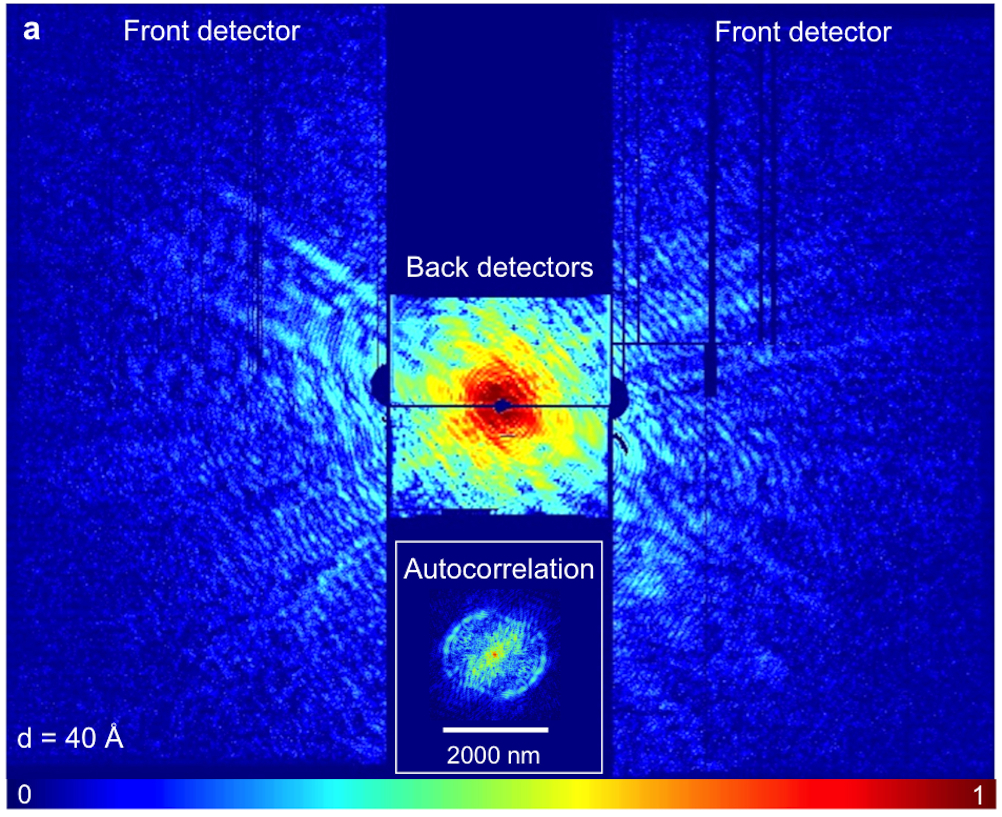
\includegraphics[width=100mm]{StrongHit.png}
	\caption{Combined diffraction signal of front and back detector. In strong hits the scattered signal from a micron-sized \textit{S. elongatus} cell extends to 4 nm full-period resolution. The size of a small molecule is 4 nm. The cell was alive during the exposure. The central area of the diffraction pattern is saturated, which prevented image reconstruction. The autocorrelation, shown in the central box, indicates the shape of the imaged cell.}\label{fig:StrongHit}
\end{figure}

\section{Data Deposition}
The ability to record millions of diffraction patterns in a day at X-ray free-electron lasers (XFELs) opens up new opportunities for experiments on cells. The massive amount of data will represent more than just individual projection images of cells. There is however a need to develop algorithms to create abstract models of cells from the data. With so many images per day, even statistically rare events could be pinpointed and studied. XFEL beam time is scarce nonetheless, and many researchers have limited access to experimental XFEL data. To aid the development of algorithms that can interpret the wealth of diffraction data we have released the data sets used in the cell study (\textbf{Paper II}). We deposited both raw and pre-processed data at the Coherent X-ray Imaging Data Bank (CXIDB) \cite{Maia2012a} (http://www.cxidb.org/id-37.html), and published a descriptor of the data that includes experimental details, as well as the structure of the deposited data, including the parameters used for data selection.

\section{RedFlamingo}

RedFlamingo has been tested on several datasets. This chapter shows four cases that illustrate different demands on the data analysis. In the first example, RedFlamingo is used for pattern classification. The main discriminatory features were size, particle elongation, and number of particles in the beam. The second example shows that RedFlamingo can be used to size particles within a wide range of sizes and shapes. The third example shows that diffraction patterns from single particles can be separated from diffraction patterns originating from multiple particles located at a distance from each other. The final example shows how the shape of elongated particles can be determined more accurately. 

\subsection{Pattern Classification of an heterogeneous RDV data set}
Rice Dwarf Virus (RDV) is the causal agent of rice dwarf disease. It can result in severe crop losses in rice and other gramineae plants in East Asian countries due to stunted growth and chlorotic specks. The structure of RDV has previously been solved to 3.5 {\AA} resolution by X-ray crystallography \cite{Nakagawa2003} (PDB 1UF2). The RDV capsid has an icosahedral symmetry, and it is approximately 72 nm in diameter across the 5-fold axis.

As part of a large international collaboration called the Single Particle Imaging initiative (SPI)\cite{Aquila2015a}, an extensive dataset of RDV hits was collected. Most diffraction patterns in this data set are not affected by detector saturation, which makes it possible to estimate the size of the icosahedral-shaped particle by determining the location of the first minima in the diffraction patterns (see Chapter 8).
RDV was classified on the size and shape of the central speckle, and the size and shape of the central term in the autocorrelation. If the central speckle and the central term of the autocorrelation are circular or only slightly elongated the particle was classified as a single particle.  

\begin{figure}[!ht]
\centering
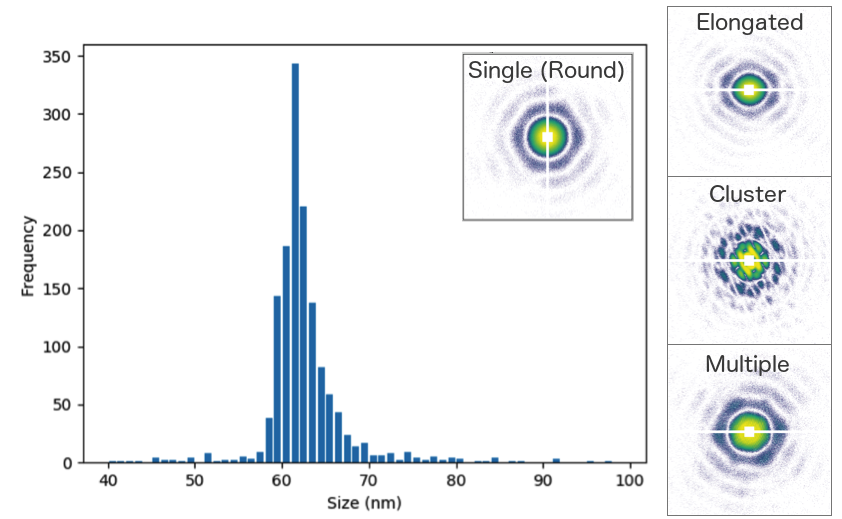
\includegraphics[width=120mm]{Chapter_09_Results_RDV.png}
\caption{Classification of particles. The size distribution of the 3608 diffraction patterns that were classified as single hits shows a peak at 63 nm. Right panels shows an  example of a diffraction pattern of each class. The gap between the two detector halves and the beam stop is masked out.}\label{fig:Classes}

\end{figure}

The diffraction patterns that have a round central speckle show features commonly associated with icosahedral particles. 

\subsection{Pattern Selection based on edges}
The second example deals with the selection of diffraction patterns based on the presence of sharp edges. The sample used was the 331-kbp chlorovirus Paramecium bursaria chlorella virus 1 (PBCV-1). PBCV-1 is the type member of the genus Chlorovirus that infects certain chlorella-like green algae from freshwater sources \cite{VanEtten2012}. It is a quasi-icosahedral particle with a diameter of 190 nm across the 5-fold axis.

In the experiment PBCV particles were injected into the XFEL focus using a GDVN. As expected for particles significantly smaller than the drop size, this resulted in a wide size distribution, of which elongation assessment showed that most particles are very round. Using the edge finding algorithm described in Chapter 8, we could find patterns that show clear features related to edges, as shown in Figure \ref{fig:PatternSelection}, separating these patterns from objects with spherical appearance.

\begin{figure}[!ht]
\centering
\includegraphics[width=120mm]{Chapter_09_Results_PBCV.png}
\caption{Measured particle size-distribution when shooting Paramecium bursaria chlorella virus 1 (PBCV-1) and xenon clusters during an X-ray holography experiment (Paper X). Sizing of hits by RedFlamingo shows a wide size distribution. Particles with a diameter of around 70 nm are likely to be Xenon-clusters. These clusters were co-injected with the PBCV particles. The peak around 170 matches the size of the PBCV particles, and the peak of particle-size 240 might be a contamination by an earlier imaged virus of approximately that size. Most particles were very spherical, but using the edge detection algorithm, patterns similar to 8.1 were selected. Six examples of such patterns are shown on the right.}\label{fig:PatternSelection}

\end{figure}


\subsection{X-ray holography on the fly - Multiple objects in the X-ray focus}

I participated in an experiment at the LCLS to capture holographic images of viruses, using two injectors simultaneously to shoot virus particles and reference objects into the X-ray beam. One of these injectors was our aerosol injector, used to inject virus particles into the X-ray focus. The other injector one was a xenon cluster source, used  to create a beam of reference objects. The cluster beam intersected the sample beam in the X-ray focus (\textbf{Paper X}). We used clusters of approximately 70 nm in diameter. A holographic diffraction pattern was recorded when the X-ray pulse simultaneously captured a sample particle and one or more reference objects. Such a pattern is similar to Figure 8.5. During the experiment, some of the hits came from single reference objects or sample particles, others from various combinations of these, including single and multiple sample particles, single and multiple reference objects, or any mixture of sample particles and reference objects. The various types of shots had to be sorted out and this was achieved by RedFlamingo, using the algorithm described in Chapter 8. Table 9.7 shows the results of the classification for samples varying between 70 and 2000 nm in size. 

\begin{figure}[!ht]
\centering
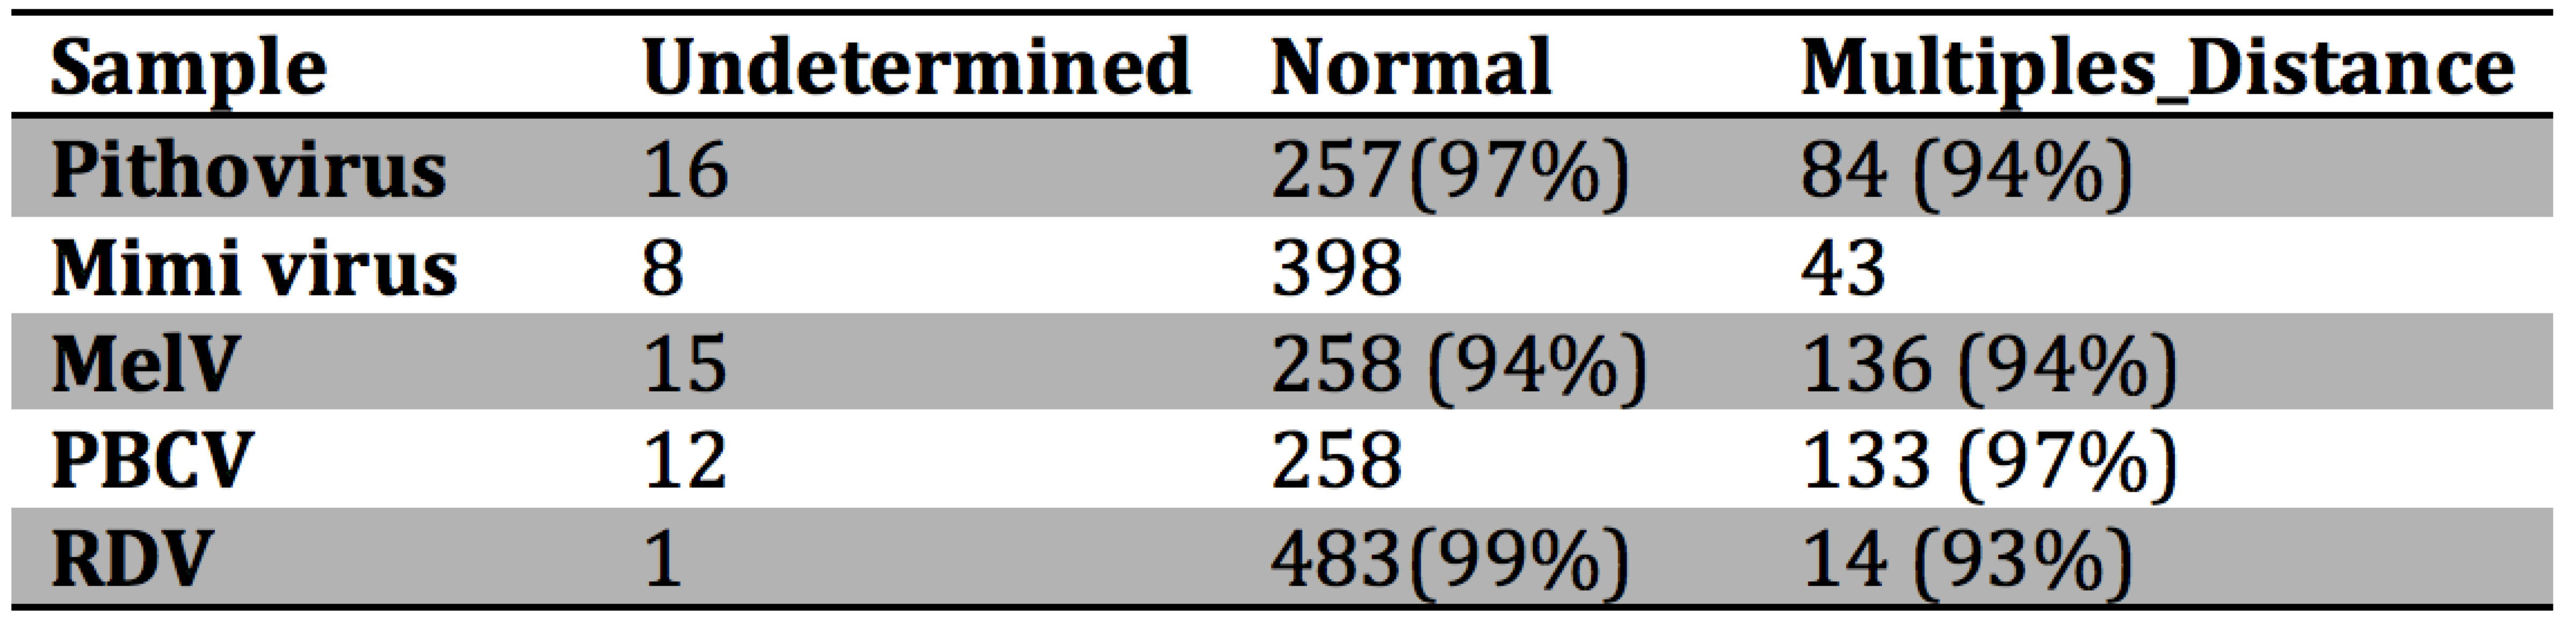
\includegraphics[width=100mm]{Chapter_09_Results_successrate.png}
\caption{Identification of multiple particles in the focus. Diffraction patterns from five different samples ranging from > 1000 nm to 70 nm in size were classified as either singles or coming from multiple particles at the same time. There are three classes: MultipleDistance, Normal, and Undetermined. Patterns with strong saturation are put in the latter class, because the autocorrelation sometimes shown strong artefacts because of it. The percentage between brackets indicates the successrate of classifying the patterns correctly in the class.}\label{fig:multiple_find}

\end{figure}

\subsection{Particle Shape Assessment}

\textit{Pithovirus sibericum} is a 30,000 year-old giant virus (about 500 nm x 2000 nm) from the Siberian permafrost and its shape resembles a “pithos”, i.e. a large amphora used by the ancient Greeks. We used RedFlamingo for the automated shape assessment of the elongated virus particle. Using the shape assessment algorithm of RedFlamingo illustrated by Figure8.4, we determined the shape of many particles. Figure 9.8 shows a scatter plot of the maximum and minimum size for each particle. The results show that a large fraction of the particles is roundish in shape. The size variations follow expectations. In the future this methods might find itself useful for the automation of the reconstruction of heterogeneous particles of unknown size, such as cells.

\begin{figure}[!ht]
\centering
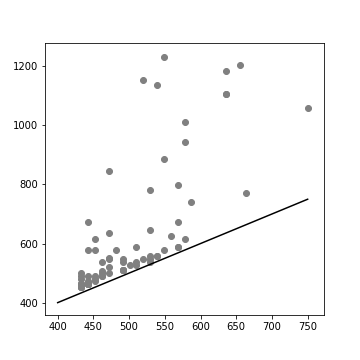
\includegraphics[width=100mm]{Chapter_09_Results_Refined_Sizing.png}
\caption{Scatter plot of the minium size of the particle vs. the maximum size of a particle, derived from the filtered autocorrelation. }\label{fig:majorminor}

\end{figure}



%\section{Software}


    \chapter{Discussion}

In synchrotron X-ray microscopy, the maximal attainable resolution on non-living biological particles is limited to about 10 nm. Unfortunately, synchrotron radiation kills live cells long before any measurable signal can be accumulated, and, as a consequence, no living cell has ever been imaged at high resolution at a synchrotron. ‘Diffraction before destruction’ overcomes this problem and can give high-resolution data, but it only permits one shot from the sample, corresponding to a spherical section through the Fourier amplitudes of the object. Three-dimensional structure determination is possible for identical objects exposed to the beam one-by-one in different orientations; this however cannot be done easily with non-identical objects, such as cells. Methods have been proposed for the simultaneous illumination of cells from multiple directions to provide a 3D view of the object, and instrumentation to achieve this is under development. However, the viewing angles are small and the views one can hope for are few. 

Although 3D imaging would be highly desirable, studies on living cells are based almost entirely on 2D images. Clinical and research laboratories around the world utilize 2D projections of cells. Features are brought out by phase-contrast techniques. We can also do that as described in this thesis.
 
According to predictions, data to sub-nanometer resolution may be recorded on micron-sized living cells through ‘diffraction- before-destruction’. Physical limits to resolution in the pattern are related to sample size and composition, pulse duration, pulse intensity, wavelength and the movement of the sample during exposure. No fundamental limit has been encountered so far with pulses presently available from the LCLS, and the results presented here are in agreement with predictions. It is, however, not trivial to image large objects, like small living cells, at high resolution.

In evaluating resolution we make a distinction between resolution in the signal and in the reconstruction. We have recorded data beyond 4 nm resolution, and reconstructed images up to a resolution of 76 nm. These are still the highest resolution recordings and reconstructions of living cells using coherent diffractive imaging. To reach nanometer resolution in reconstructions, we need to meet certain requirements.

The diffraction signal fades away with an exponent of  about 3.31 over the range of spatial frequencies probed in our measurements. Accurate measurement of nanometer signal requires very low background. Container-free sample injection delivers truly isolated samples into the X-ray beam to record diffraction patterns with low scattered background. Under these conditions, signal from the sample can be measured to the highest possible resolution over a flat background. The contrast between the sample and its surrounding (wet helium gas expanding into a vacuum chamber) is high. The clean background and the high contrast are important for the finite support constraint in phase retrieval. We estimate that nanometer resolution in the signal of a micron-sized cell would require a pulse with duration shorter than 10fs and around $10^{12}$–$10^{13}$ photons on a micron-sized sample at 3-10 keV photon energy.

Resolution in a 2D reconstruction from a single exposure depends on the success of phase retrieval, and is also influenced by the lift-off of the Ewald sphere from the projection plane at high angles (shorter wavelengths would alleviate this problem). The projection approximation also presumes that the Born approximation is valid. This requires harder X-rays for samples thicker than those studied here.

The maximal size of an object for successful reconstruction is currently limited to about 1-2 micron at the LCLS for a number of reasons. 
First, the bandwidth of an LCLS pulse is about 0.2\% and this gives about 500 resolution elements in an image. If a target resolution of 2 nm is aimed for, the object size cannot be bigger than about 1 micron. Smaller bandwidth would allow studies on larger objects. An oversampled diffraction pattern is necessary for phase retrieval. 
Second, the focus must be large enough to cover the sample yet contain enough photons to produce strong scattered signal from the cell. A larger focus requires more photons per pulse and these extra photons are currently not available from the LCLS. This limits the maximal useful focus size, which in turn limits the object size to about 1-2 micron.

Missing low-resolution data pose perhaps the largest problem in image reconstruction. Low-resolution terms are crucial for the determination of the support for the object. The X-ray detector has a hole at its centre to let the direct beam pass through. The size of this blind spot limits the maximal object size to 1-2 um at the relevant wavelengths. In strong exposures, there is a further and significant loss of low-resolution data due to detector saturation.

The current limitations are technical. A femtosecond exposure ‘freezes’ all cellular processes at room temperature, including diffusion, and thus eliminates blurring. This is an advantage over other cell-imaging methods and will become important if or when nanometer/subnanometer resolution will be achieved on a micron-sized cell. At the moment, the LCLS is still too weak. This is illustrated in Figure .


\begin{figure}[!h]
\centering
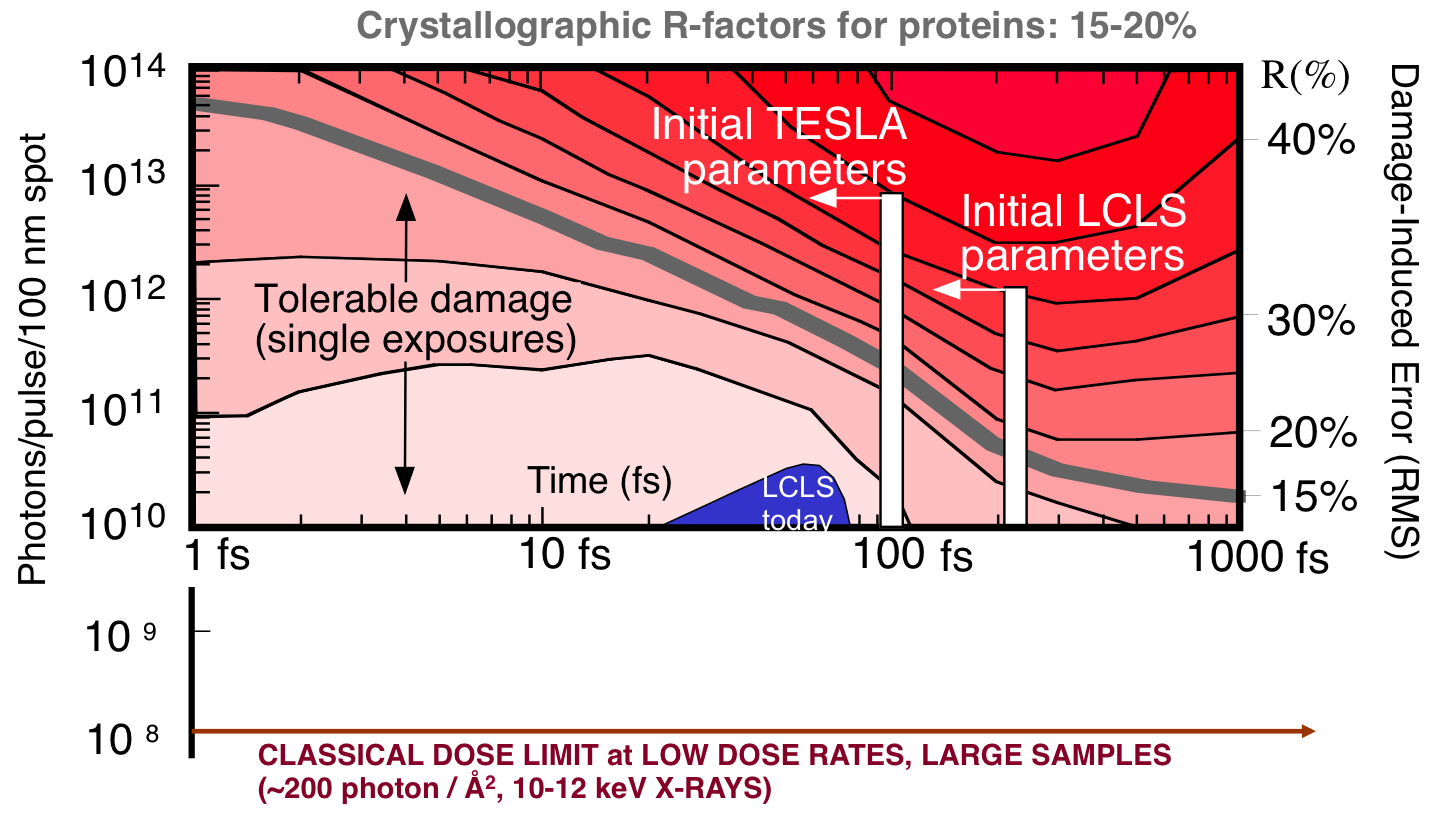
\includegraphics[width=120mm]{Chapter_10_Discussion_LandscapeDamageTolerance.png}
\caption{The landscape of damage tolerance. Contour plots of the weighted electronic R factors [from equation (2) in \cite{Neutze2000}] as functions of the X-ray  flux and pulse duration at 12 keV photon energy. The plot illustrates the extent to which the information content of the elastically scattered X-rays is degraded by radiation damage. Damage as regarded acceptable if the R-factor is below 15\%,  indicated by the grey line. Photon pulses from the LCLS are weak, and have not reached the grey line anywhere in the parameter space.}\label{fig:landscape}
\end{figure}

No fundamental limit has been encountered at free-electron lasers so far, and exciting new science is still to come. Stronger and shorter pulses, like those expected from the European XFEL could bring high-resolution cellular imaging within reach. 
	
	%\chapter{Sammanfattning pa Svenska}

In this thesis we want to develop new methods to image biological diversity at the molecular level. Understanding this diversity is very important as it can play a major role in development of deceases. The thesis focuses on two topics: the imaging \textit{living} cells and the development of a computational tool to assess variability within a population of images.
\\\\
In molecular biology structure and function are closely related. This however does not mean that each object has one single static shape. On the contrary, many objects have multiple conformations and only through understanding the variation, their function becomes interpretable. A further complication arises from the fact that the variation is often highly dependent on the exact environment the objects are in. Outside of their natural environment, molecular machines might start operating differently. A tool that could image molecular machinery inside their natural environment, the living cell, is therefore required for us to truly understand the structure of molecular life.
\\\\
The amount of detail we can image in an object is limited to about the size of the wavelength of the light used. Molecular machines are build up out of atoms, so light with a wavelength similar to the size of an atom is needed to see single atoms and thus understand the functioning of molecular machines fully. This type of light is called X-ray radiation. Another fundamental principle is that the smaller an object is, the stronger light is needed in order to record enough information to record an image. Strong beams however have the disadvantage that they damage the objects themselves. This leads to the limitation that single objects smaller than 100 atoms in diameter can not be visualized using ordinary techniques.
\\\\
The development of a new type of X-ray laser called an x-ray free-electron lasers, that produces ultra short and extremely bright X-ray pulses might hold the solution to this limit imposed by sample damage. The power of the pulse ensures that even individual molecular machines can be imaged in atomic detail. These pulses do damage the sample, but because they are ultra-short the damage only happens after the pulse has passed. The recorded image is therefore an image of the undamaged object. This principle is called diffraction before destruction. 
\\\\
The word diffract indicates that we are not recording images of an object in the same way that a photo camera captures images. Instead we measure a so called diffraction pattern. The 2D diffraction pattern can be converted to a real image (2D) in a process called image reconstruction. The feasibility of diffraction before destruction and the image reconstruction process has been shown for a variety of non-biological and biological samples in 2D.  And recently the first 3D model of a biological object has been generated from many diffraction patterns generated using this method.
\\\\
In 2008, researchers showed that it is theoretically possible to image small living cells at sub-nanometer resolution in 2D. The main work of the thesis was an experimental verification of this prediction. This study showed that using an XFEL that was weak compared to the imaginary ones used in the predictions, it is possible to record images with signal up to 4 nm resolution which is equivalent to 40 atomic diameters. The problem of these images is that the strong signal caused the detector to saturate. We therefore had to resort to weaker diffraction patterns for the analysis. This posed the limit on the resolution of the recovered object. We have suggested improvements to avoid detector saturation, but these suggestions have not yet been tested experimentally.
\\\\
Due to the variability between different cells it is not trivial to fully automate the process of object reconstruction from the recorded diffraction, something that is needed to study the variability of cells in high detail, or the molecular machines inside of them. For the automation to succeed it necessary to predict the shape of the object from the recorded image itself. Furthermore, other parameters such as saturation or having two cells in the beam at once also have to automatically identified.
\\\\
This led to the development of the software suite called RedFlamingo. RedFlamingo can be used to assess the quality of individual images and deduces several essential features for image reconstruction. In some cases it can also determine whether the observed variety originate from a biological source, or whether it is a result from he experiment. It turns out that this feature can be useful in the process of deriving a 3D model from many 2D images. 
\\\\
I am very excited to be part of the development of this technique. Measuring images without saturation effects might open the door to observing the biological processes occurring inside living cells. For the future I see the study of variability in isolated molecular machines as the first milestone. After that I hope that these machines can be studied together with their natural environment, allowing us to visualize the organisation of life.

	%\chapter*{Acknowledgements}




\chapter*{Author Contribution}

\section*{Paper I}
I performed the data analysis, excluding the preprocessing. That includes the pattern selection, phase recovery, missing mode analysis, and the clustering analysis.

\section*{Paper II}
I performed the data analysis, including the preprocessing and the pattern selection.

\section*{Paper III}
I performed the data analysis, including the preprocessing, hit selection, and pattern classification. For the latter we used a software package I wrote.

	
\backmatter
    % References
    % No restriction is set to the reference styles
    % Save your references in References.bib
    \nocite{*} % Remove this for your own citations
    \bibliographystyle{ieeetr}
    \bibliography{Thesis}

\end{document}